%versi 2 (8-10-2016)

\chapter{Landasan Teori}
\label{chap:teori}

\section{Persamaan Diferensial}
\label{sec:PD} 
 
Persamaan diferensial adalah suatu persamaan matematika yang mengandung turunan-turunan dari suatu fungsi yang tidak diketahui (\begin{math} y(x) \end{math}) dari satu atau lebih variabel bebas terhadap satu atau lebih peubah tak bebas. Di dalam aplikasi di dunia nyata,
fungsi yang tidak diketahui tersebut digunakan untuk merepresentasikan perubahan secara kontinu. Turunan-turunan fungsi merepresentasikan laju perubahan. Persamaan diferensial merepresentasikan hubungan antar fungsi dan turunan. Hubungan antar fungsi dan turunan
tersebut atau persamaan diferensial memegang peranan penting dalam berbagai bidang disiplin ilmu seperti fisika (hukum Newton), kimia (hukum Bernoulli), biologi (laju pertumbuhan bakteri), ekonomi, dan lain-lain.

Contoh persamaan diferensial adalah sebagai berikut:

\begin{enumerate}

	\item \begin{math} \dfrac{\, d^{2}y}{\, dx^{2}} + xy(\dfrac{\, dy}{\, dx})^{2} = 0 \end{math} (persamaan diferensial dengan peubah tak bebas \textit{y} dan peubah bebas \textit{x})
	\item \begin{math} \dfrac{\, d^{2}x}{\, dt^{2}} + \dfrac{\, dx}{\, dt} - 5\cos t + 2x = 0 \end{math} (persamaan diferensial dengan peubah tak bebas \textit{x} dan peubah bebas \textit{t})
	\item \begin{math} \dfrac{\, d^{2}u}{\, dy^{2}} + u^{2}y = 0 \end{math} (persamaan diferensial dengan peubah tak bebas \textit{u} dan peubah bebas \textit{y})
	\item \begin{math} \dfrac{\partial v}{\partial x} + \dfrac{\partial v}{\partial y} = xy \end{math} (persamaan diferensial dengan peubah tak bebas \textit{v} dan peubah bebas \textit{x} dan \textit{y})
	\item \begin{math} \dfrac{\partial v}{\partial x} + \dfrac{\partial u}{\partial t} + \dfrac{\partial v}{\partial t} + \dfrac{\partial u}{\partial x}= 3 \end{math} (persamaan diferensial dengan peubah tak bebas \textit{v} dan \textit{u} dan peubah bebas \textit{x} dan 	 \textit{y})
	
\end{enumerate}

Persamaan diferensial memiliki orde (tingkat) dan turunan. Orde persamaan diferensial adalah \textit{n} jika turunan (\textit{y}) ke-\textit{n}-nya merupakan turunan tertinggi. Derajat persamaan diferensial adalah pangkat tertinggi dari turunan tertinggi persamaan diferensial tersebut.

Contoh orde dan turunan pada persamaan diferensial adalah sebagai berikut:

\begin{enumerate}

	\item \begin{math} 2\dfrac{\, dy}{\, dx} + y = x^{3} \end{math} (persamaan diferensial orde 1 derajat 1)
	\item \begin{math} y'''+ 2(y'')^{2} + y' = \tan x \end{math} (persamaan diferensial orde 3 derajat 1)
	\item \begin{math} y^{iv} + y''' + y = \ln x \end{math}  (persamaan diferensial orde 4 derajat 1)
	\item \begin{math} y^{2}y' + x = 0 \end{math} (persamaan diferensial orde 1 derajat 2)
	\item \begin{math} y'' + xy(y')^{3} = 0 \end{math}  (persamaan diferensial orde 2 derajat 4)
	
\end{enumerate}

Solusi persamaan diferensial dapat dicari dan ditemukan dengan menggunakan metode analitik (menggunakan rumus-rumus matematika yang sudah baku) dan metode numerik (menggunakan bantuan formulasi matematis pada program komputer). Solusi dengan metode analitik
akan berupa sebuah fungsi eksak dan solusi dengan metode numerik akan berupa hamparan (\textit{range}) angka. Dalam skripsi ini, solusi persamaan diferensial akan dicari dan ditemukan dengan metode analitik karena keluaran perangkat lunak akan berbentuk fungsi matematika yang eksak. 

Persamaan diferensial dibagi menjadi dua berdasarkan jumlah peubah bebas dan jumlah peubah tak bebasnya, yaitu persamaan diferensial biasa dan persamaan diferensial parsial. Persamaan diferensial biasa adalah persamaan diferensial yang memiliki tepat satu buah peubah
bebas dan tepat satu buah peubah tak bebas. Persamaan diferensial parsial adalah persamaan diferensial yang memiliki satu buah atau lebih peubah bebas dan satu buah atau lebih peubah tak bebas.

\subsection{Aturan Turunan Fungsi}
\label{sec: rules}

Seperti yang sudah dijelaskan pada bag 2.1, persamaan diferensial memuat turunan-turunan dari suatu fungsi yang tidak diketahui. Turunan-turunan tersebut memiliki aturan berupa rumus-rumus untuk menemukan fungsi yang tidak diketahui tersebut. Berikut adalah aturan
turunan fungsi:

\begin{enumerate}[1.]

	\item Aturan turunan fungsi aljabar tunggal

		\begin{itemize}

			\item Jika \begin{math} f(x) = k \end{math} dengan \begin{math} k \end{math} = konstanta riil, maka turunan \begin{math} f(x) \end{math} adalah \begin{math} f'(x) = 0 \end{math}
			\item Jika \begin{math} f(x) = x \end{math} (fungsi identitas), maka \begin{math} f'(x) = 1 \end{math}
			\item Jika \begin{math} f(x) = ax^{n} \end{math}, dengan \begin{math} a \end{math} adalah konstanta riil tidak nol dan \begin{math} n\end{math} merupakan bilangan bulat positif, maka \begin{math} f'(x) = a.n.x^{n-1} \end{math}

		\end{itemize}

	\item Aturan turunan fungsi aljabar ganda
	\\
	\\
	Misalkan \begin{math} u(x) \end{math} dan \begin{math} v(x) \end{math} masing-masing mempunyai turunan \begin{math} u'(x) \end{math} dan \begin{math} v'(x) \end{math}
	
		\begin{itemize}

			\item Jika  \begin{math} f(x) =  u(x) \pm v(x) \end{math}, maka  \begin{math} f'(x) =  u'(x) \pm v'(x) \end{math}
			\item Jika  \begin{math} f(x) =  u(x).v(x) \end{math}, maka \begin{math} f'(x) =  u'(x).v(x) + u(x).v'(x) \end{math}
			\item Jika  \begin{math} f(x) = \dfrac{u(x)}{v(x)}, v(x) \neq 0 \end{math}, maka  \begin{math} f'(x) = \dfrac{u'(x).v(x) - u(x).v'(x)}{(v'(x))^{2}} \end{math}

		\end{itemize}

	\item Aturan turunan fungsi aljabar berpangkat \textit{N}

		\begin{itemize}

			\item Jika \begin{math} f(x) = (u(x))^{n} \pm v(x) \end{math}, dengan \begin{math} u(x) \end{math} adalah fungsi dari \begin{math} x \end{math} yang mempunyai turunan \begin{math} u'(x) \end{math} dan \begin{math} n \end{math} adalah
			bilangan riil, maka \begin{math} f'(x) = n.(u(x))^{n-1}.u'(x) \end{math}

		\end{itemize}

	\item Aturan turunan fungsi trigonometri

		\begin{itemize}

			\item Jika \begin{math} f(x) = \sin x \end{math}, maka turunannya adalah \begin{math} f'(x) = \cos x \end{math}
			\item Jika \begin{math} f(x) = \cos x \end{math}, maka turunannya adalah \begin{math} f'(x) = -\sin x \end{math}
			\item Jika \begin{math} f(x) = \sin x \end{math}, maka turunannya adalah \begin{math} f'(x) = \sec^{2} x \end{math}
			\item Jika \begin{math} f(x) = \csc x \end{math}, maka turunannya adalah \begin{math} f'(x) = -\csc x.\cot x \end{math}
			\item Jika \begin{math} f(x) = \sec x \end{math}, maka turunannya adalah \begin{math} f'(x) = \sec x.\tan x \end{math}
			\item Jika \begin{math} f(x) = \cot x \end{math}, maka turunannya adalah \begin{math} f'(x) = -\csc^{2} x \end{math}

		\end{itemize}

\end{enumerate}

\subsection{Solusi Persamaan Diferensial}
\label{sec:solusi}

Solusi persamaan diferensial adalah suatu fungsi matematika (\begin{math} f(x) \end{math}) atau keluarga fungsi yang menjadi fungsi yang tepat untuk memenuhi fungsi yang tidak diketahui (\begin{math} y \end{math}) dalam persamaan diferensial. Jika \begin{math} f(x) \end{math} disubstitusikan untuk \begin{math} y \end{math} dalam persamaan diferensial, maka akan menghasilkan suatu fungsi yang benar. Solusi persamaan diferensial terbagi atas solusi umum dan solusi khusus.

Solusi umum persamaan diferensial adalah suatu fungsi matematika (\begin{math} f(x) \end{math}) yang memuat atau mengandung beberapa parameter dan memenuhi persamaan diferensialnya. Banyaknya parameter dalam solusi umum sama dengan orde persamaan diferensialnya. Contoh solusi umum persamaan diferensial adalah sebagai berikut:

\begin{enumerate}[1.]

	\item aa

\end{enumerate}

Solusi khusus persamaan diferensial adalah fungsi matematika (\begin{math} f(x) \end{math}) yang merupakan anggota dari keluarga fungsi solusi umum persamaan diferensialnya. Solusi khusus diperoleh dengan mensubstitusikan parameter pada solusi umum oleh suatu konstanta. Contoh solusi khusus persamaan diferensial adalah sebagai berikut:

\subsection{Persamaan Diferensial Biasa}
\label{sec:PDB}

Persamaan diferensial biasa adalah persamaan diferensial yang memiliki tepat satu buah peubah bebas dan tepat satu buah peubah tidak bebas. Persamaan diferensial biasa memegang peranan penting dalam hal menurunkan fungsi-fungsi yang tidak diketahui dalam beberapa
aplikasi dalam bidang fisika (hukum Newton), biologi (laju pertumbuhan bakteri), dan lain-lain. Persamaan diferensial biasa yang bersifat linier dapat dipecahkan dengan metode analitik, sementara persamaan diferensial biasa yang bersifat non-linier sulit dipecahkan dengan 
metode analitik, sehingga harus menggunakan bantuan komputasi program komputer (dengan bantuan metode numerik). Cakupan bahasan skripsi ini hanya sampai pada persamaan diferensial biasa linier. 

Persamaan diferensial biasa memiliki fungsi-fungsi turunan yang tidak diketahui berupa \begin{math} y = g(x) \end{math}. Fungsi \begin{math} y \end{math} merupakan solusi persamaan diferensial biasa apabila \begin{math} g(x) \end{math} dapat diferensialkan sehingga persamaan tersebut menjadi solusi tunggal (identitas) pada persamaan tersebut. Hal utama dalam persamaan diferensial biasa adalah mencari semua solusi persamaan yang diberikan. 

Langkah-langkah untuk menentukan solusi persamaan diferensial biasa adalah sebagai berikut:

\begin{enumerate}[1.]

	\item Tentukan banyaknya konstanta sembarang (\begin{math} y^{n} \end{math})
	\item Turunkan sebanyak konstanta sembarangnya sampai menjadi sebuah fungsi (solusi)
	\item Jika solusi hasil turunan tersebut didiferensialkan sehingga konstanta sembarangnya sudah lenyap maka hasil diferensialnya merupakan persamaan diferensial biasa
	\item Jika konstanta sembarangnya masih ada maka eliminasi konstanta sembarangnya sampai tidak ada
	
\end{enumerate}

Klasifikasi persamaan diferensial biasa adalah sebagai berikut:

\begin{enumerate}[1.]
	
	\item Homogen
	\\
	Persamaan diferensial biasa homogen adalah persamaan diferensial biasa yang memiliki bentuk \begin{equation} a_0(x)y^{n} + a_1(x)y^{n - 1} + ... + a_n-1(x)y' + a_n(x)y = 0 \end{equation}  pada orde \textit{N}.
	\\
	\item Non-homogen
	\\
	Persamaan diferensial biasa non-homogen adalah persamaan diferensial biasa yang tidak memiliki bentuk seperti persamaan 2.1
	\\
	\item Linier	
	\\
	Persamaan diferensial biasa linier adalah persamaan diferensial biasa yang memiliki bentuk \begin{equation} a_0(x)y^{n} + a_1(x)y^{n - 1} + ... + a_n-1(x)y' + a_n(x)y = f(x) \end{equation} pada orde \textit{N}.
	\\
	\\
	Kriteria-kriteria persamaan diferensial biasa linier adalah:

	\begin{enumerate}[1.]

		\item Tidak terdapat perkalian antara peubah bebas dan peubah tak bebas
		\item Tidak terdapat fungsi transeden dalam peubah tak bebas
		\item Peubah tak bebas dan turunannya paling besar berpangkat satu
		\item \begin{math} a_i(x) \end{math} , di mana \begin{math} i = 0, 1, 2, ... \end{math} masing-masing merupakan fungsi kontinu dalam \begin{math} x \end{math} pada suatu interval 

	\end{enumerate}

	Contoh persamaan diferensial biasa linier (dalam skripsi ini persamaan diferensial biasa linier yang akan langsung dibahas adalah persamaan diferensial biasa linier orde dua):

	\begin{enumerate}[1.]

		\item \begin{math} x (\dfrac{\, d^{2}y}{\, dx^{2}}) + 3 \dfrac{\, dy}{\, dx} - 2xy = 0 \end{math}
		\item \begin{math} (\cos x) y" + (\sin x)y' + 4y \tan x = 0 \end{math}
		\item \begin{math} xy'' + 3y' - x^{2}y = e^{x}\end{math}
		\item \begin{math} y^{iv}+ x^{2}y'' + x^{3}y' = 0 \end{math}
		\item \begin{math} (x^{2} - 1) y" + (x+1) y' + 2y = 0 \end{math}

	\end{enumerate}

	\item Non-linier
	\\
	Persamaan diferensial biasa non-linier adalah persamaan diferensial biasa yang tidak memiliki bentuk seperti persamaan 2.2.
	\\
	Contoh persamaan diferensial biasa non-linier:

	\begin{enumerate}[1.]

		\item \begin{math} y (\dfrac{\, d^{2}y}{\, dx^{2}}) + x (\dfrac{\, dy}{\, dx})^{2} - 4x = \cos x \end{math}
		\item \begin{math} y" + 6yy' + 4xy = 0 \end{math}
		\item \begin{math} x (y")^{2} + x^{2} y' - 2y = 0\end{math}
		\item \begin{math} y' \sin x - x \sin y = 7x \end{math}
		\item \begin{math} y" - 2xy + 3 \cos y = 0 \end{math}

	\end{enumerate}

\end{enumerate}

Berikut akan dibahas persamaan diferensial biasa homogen dan persamaan diferensial biasa non-homogen. Di bawah ini adalah jenis-jenis persamaan diferensial biasa homogen, selanjutnya akan dibahas persamaan diferensial biasa non-homogen.

\subsubsection{Persamaan Diferensial Biasa Orde Satu Derajat Satu}
\label{par:PDB1}

Bentuk umum persamaan diferensial biasa orde satu derajat satu dapat ditulis dalam bentuk:

\begin{equation} M(x,y) \, dx + N(x, y) \, dy = 0 \end{equation}

Bentuk ini dapat dimanipulasi menjadi bentuk lain dengan pengertian yang sama dengan bentuk:

\begin{displaymath} (y + x) \, dx + (y - x) \, dy = 0 \end{displaymath}

Dari hasil manipulasi terlihat bahwa:

\begin{displaymath} M(x, y) = (y + x),  N(x, y) = (y - x) \end{displaymath}

Bentuk di atas dapat pula ditulis menjadi:

\begin{displaymath} \dfrac{\, dy}{\, dx} + \dfrac{y + x}{y - x} \end{displaymath}

Persamaan diferensial biasa orde satu derajat satu dapat diselesaikan dengan menggunakan beberapa metode. Metode-metode ini adalah:

\paragraph{Memisahkan Peubah}
\label{par:MP}

Bentuk \begin{math} M(x, y) \, dx + N(x, y) \, dy = 0 \end{math} dapat diubah menjadi \begin{math} P(x) \, dx + Q(y) \, dy = 0 \end{math} di mana \begin{math} P(x) \end{math} adalah suatu fungsi dari konstanta \begin{math} x \end{math} saja dan \begin{math} Q(y) \end{math} adalah suatu fungsi dari konstanta \begin{math} y \end{math} saja. Persamaan dengan bentuk tersebut dinamakan persamaan dengan peubah terpisah (memisahkan peubah). Dengan mengintegralkan kedua ruas (\begin{math} P(x) \end{math} dan \begin{math} Q(y) \end{math}), maka diperoleh:

\begin{equation} \int P(x) \, dx + \int Q(y) \, dy = 0 \end{equation}

Jika diasumsikan bahwa \begin{math} P \end{math} dan \begin{math} Q \end{math} adalah fungsi yang kontinu, maka persamaan 2.3 dapat dihitung dan diperoleh solusi umum dan khusus-nya.

Contoh kasus persamaan diferensial biasa yang dapat diselesaikan dengan metode memisahkan peubah adalah:

\begin{enumerate}[1.]

	\item \begin{math} yy' + 4x = 0 \end{math}\\ \\
	         \begin{math} y \dfrac{\, dy}{\, dx} + 4x = 0 \end{math}\\ \\
	         \begin{math} y \, dy + 4x \, dx = 0 \end{math}\\ \\
	         \begin{math} \int y \, dy + \int 4x \, dx = \int 0 \end{math}\\ \\
	         \begin{math} \dfrac{1}{2}y^{2} + 2x^{2} = C \end{math}\\ \\
	         \begin{math} y^{2} = C - 4x^{2} \end{math}\\ \\
	         \begin{math} y = \sqrt{C - 4x^{2}}\end{math}
	         
	\item \begin{math} y' = 1 + y^{2} \end{math} \\ \\
	         \begin{math} \dfrac{\, dy}{\, dx} + 4x = 0 \end{math}\\ \\
	         \begin{math} \dfrac{\, dy}{1 + y^{2}} = \, dx \end{math}\\ \\
	         \begin{math} \int \dfrac{\, dy}{1 + y^{2}} = \int \, dx \end{math}\\ \\
	         \begin{math}\arctan(y) = x + C \end{math}\\ \\
	         \begin{math} y = \tan (x + C) \end{math}

\end{enumerate}

\paragraph{PDB Homogen}
\label{par:PDBHomo}

Bentuk \begin{math} M(x, y) \, dx + N(x, y) \, dy = 0 \end{math} adalah persamaan diferensial biasa homogen apabila \begin{math} M(x, y) \end{math} dan \begin{math} N(x, y) \end{math} berderajat sama. Contoh persamaan diferensial biasa homogen adalah:

\begin{enumerate}[1.]

	\item \begin{math} y = x^{3} - 2x^{2}y \end{math} (persamaan diferensial biasa homogen berderajat 3)
	\item \begin{math} y = x^{2} - 3xy^{2} \end{math} (persamaan diferensial biasa non-homogen)

\end{enumerate}

Persamaan diferensial dapat diselesaikan dengan cara substitusi:

\begin{displaymath} v = \dfrac{y}{x} \end{displaymath}
\begin{displaymath} y = vx \end{displaymath}

sehingga diperoleh:

\begin{equation} \, dy = v \, dx + x \, dv \end{equation}

Contoh kasus persamaan diferensial biasa homogen adalah:

\begin{enumerate}[1.]

	\item \begin{math}(x + y) \, dx + (y - x) \, dy = 0 \end{math}\\ \\
	         \begin{math} \dfrac{\, dy}{\, dx} = - \dfrac{x + y}{y - x} = \dfrac{x + y}{x - y} \end{math}\\ \\
	         \begin{math} \dfrac{\, dy}{\, dx} = \dfrac{1 + \dfrac{y}{x}}{1 - \dfrac{y}{x}} \end{math} (misalkan \begin{math} y =vx \end{math}, sehingga \begin{math} \, dy = v \,dx + x \, dv \end{math}) \\ \\ 
	         \begin{math} v + x  \dfrac{\, dv}{\, dx} = \dfrac{1 + v}{1 - v} \end{math}\\ \\
	         \begin{math} x \dfrac{\, dv}{\, dx} = \dfrac{1 + v}{1 - v} - v \end{math}\\ \\
 	         \begin{math} x \dfrac{\, dv}{\, dx} = \dfrac{1 + v - v(1 - v)}{1 - v} \end{math}\\ \\
	         \begin{math} x \dfrac{\, dv}{\, dx} = \dfrac{1 + v^{2}}{1 - v} \end{math}\\ \\
	         \begin{math} \dfrac{\, dv}{dx} = \dfrac{1 + v^{2}}{1 - v} \end{math}\\ \\
	         \begin{math} \dfrac{1 - v}{1 + v^{2}} \, dv = \dfrac{\, dx}{x} \end{math}\\ \\
                    \begin{math} \int \dfrac{1}{1 + v^{2}} \, dv - \int \dfrac{v}{1 + v^{2}} \, dv = \int \dfrac{1}{x} \, dx \end{math}\\ \\
	         \begin{math} \arctan(v) - \dfrac{1}{2} \ln (1 + v^{2}) = \ln x + C \end{math} \\ \\
                    \begin{math} \arctan(v) = \ln (1 + v^{2})^{\frac{1}{2}} + \ln x + C \end{math} \\ \\
                    \begin{math} \arctan(\dfrac{y}{x}) = \ln x (1 + \dfrac{y^{2}}{x^{2}})^{\frac{1}{2}} + C \end{math} 

\end{enumerate}

\paragraph{Persamaan Diferensial Biasa dengan Koefisien Linier}
\label{par:PDBKL}

Bentuk umum persamaan diferensial biasa dengan koefisien linier adalah:

\begin{equation} (ax + by + c) \, dx + (px + qy + r) \, dy = 0 \end{equation}

Metode-metode penyelesaian  persamaan diferensial biasa dengan koefisien linier adalah sebagai berikut:

\begin{enumerate}[1.]

	\item Bila \begin{math} c = 0 \end{math} dan \begin{math} r = 0 \end{math}, maka bentuk persamaan 2.6 menjadi:

	         \begin{equation} (ax + by) \, dx + (px + qy) \,dy = 0 \end{equation},

	         adalah persamaan diferensial biasa homogen sehingga dapat diselesaikan dengan mensubstitusikan \begin{math} v = \dfrac{y}{x} \end{math} 

	\item Bila \begin{math} px + qy = k (ax + by) \end{math}, di mana \begin{math} k \end{math} adalah konstanta, maka bentuk persamaan 2.6 menjadi:

                   \begin{equation} (ax + by + c) \, dx + k (ax + by) + r \,dy = 0 \end{equation},

                   Misalkan \begin{math} ax + by = z \end{math}, sehingga diperoleh \begin{math} a \, dx + b \, dy = \, dz \end{math} dan \begin{math} \, dy = \dfrac{\, dz - a \, dx}{b} \end{math}
	        \\
                   Akibatnya bentuk 2.8 menjadi:
  
	        \begin{math} (z + c) \,dx + (kz + r) \, dy = 0 \end{math} \\ \\
                   \begin{math}  (z + c) \,dx + (kz + r)  \dfrac{\, dz - a \, dx}{b} = 0 \end{math} \\ \\
                   \begin{math} b (z+ c) \,dx + (kz + r) \, dz - a (kz + r) \,dx  0 \end{math} \\ \\
                   \begin{math} b (z + c) - a (kz + r) \, dx + (kz + r) \, dz = 0 \end{math} (persamaan diferensial biasa dengan variabel terpisah)

	\item Bila \begin{math} \dfrac{a}{p} \neq \dfrac{b}{q} \end{math}  dan \begin{math} r \neq 0 \end{math}, dapat diselesaikan dengan memisalkan:
                   \\ \\
	        \begin{math} ax + by + c = u \end{math} \\ \\
                   \begin{math} px + qy + r = v \end{math} \\ \\
                   \begin{math} a \,dx + b \, dy = \, du \end{math} \\ \\
                   \begin{math} p \,dx + q \, dy = \, dy \end{math} \\ \\
        	        \begin{math} \, dx = \dfrac{
 		 \begin{vmatrix}
    			\, du & b \\
   			\, dv & q
		\end{vmatrix}
		}
  		 {
   		\begin{vmatrix}
    			a & b \\
   			p & q
   		\end{vmatrix}
   			 } = \dfrac{q \, du - b \, dy}{aq - bp}
	        \end{math} \\

Substitusi pada persamaan 2.8, maka diperoleh persamaan diferensial homogen.

\end{enumerate}

Contoh-contoh kasus persamaan diferensial biasa dengan koefisien linier adalah:

\begin{enumerate}[1.]

	\item \begin{math} (x + y + 1) \, dx + (2x + 2y + 1) \, dy = 0 \end{math} \\ \\ 
	          Misalkan \begin{math} x + y = z \end{math} , sehingga \\ \\
                    \begin{math} \, dz = \, dx + \, dy \end{math} atau \begin{math} \, dy = \, dz - \, dx \end{math} \\ \\
                     Persamaan menjadi: \\ \\
	         \begin{math} (z + 1) \, dx + (2z + 1) (\,dz - \,dx) = 0 \end{math} \\ \\
                    \begin{math} (z + 1) \, dx + (2z + 1) \, dz - (2z + 1) \, dx = 0 \end{math} \\ \\
 	         \begin{math} (2z + 1) \, dz - z \, dx = 0 \end{math} \\ \\
                    \begin{math} \int \, dx = \int \dfrac{2z+1}{2} \, dz \end{math} \\ \\
                    \begin{math} x = 2z + \ln z + C \end{math} \\ \\
	         \begin{math} x = 2 (x + y) + \ln (x+ y) + C \end{math}
		
\end{enumerate}

\paragraph{Persamaan Diferensial Biasa Eksak}
\label{par:PDBE}

Suatu persamaan diferensial biasa orde pertama berbentuk \begin{math} M(x,y) \, dx + N(x, y) \, dy = 0 \end{math} dikatakan eksak jika ruas kiri persamaan total atau diferensial eksak (\begin{math} \, du = \dfrac{\partial u}{\partial x} \, dx + \dfrac{\partial u}{\partial y} \, dy\end{math}) dari fungsi \begin{math} u(x, y) \end{math}, maka \begin{math} M(x,y) \, dx + N(x, y) \, dy = 0 \end{math} dapat ditulis menjadi \begin{math} \, du = 0 \end{math}. Dengan melakukan pengintegralan, maka diperoleh penyelesaian umum persamaan diferensial biasa orde pertama tersebut dalam bentuk:

\begin{displaymath} u(x, y) = 0 \end{displaymath}

Dengan membandingkan \begin{math} M(x, y) \, dx + N(x, y) \, dy = 0 \end{math} dan persamaan yang berikutnya, terlihat bahwa persamaan \begin{math} u(x, y) = 0 \end{math}, terlihat bahwa persamaan \begin{math} u(x, y) = 0 \end{math} adalah persamaan yang eksak
jika terdapat suatu fungsi \begin{math} u(x, y) = 0 \end{math} sedemikian sehingga:

\begin{displaymath} \dfrac{\partial u}{\partial x} = M \end{displaymath} dan \begin{displaymath} \dfrac{\partial u}{\partial y} = N \end{displaymath}

Misalkan \begin{math} M \end{math} dan \begin{math} N \end{math} terdefinisi dan mempunyai turunan parsial yang pertama dan kontinu pada suatu daerah di bidang \begin{math} xy \end{math} yang dibatasi oleh suatu kurva tertutup yang tak beririsan dengan dirinya sendiri.
Maka diperoleh turunan sebagai berikut:

\begin{displaymath} \dfrac{\partial M}{\partial y} = \dfrac{\partial^{2} u}{\partial y \partial x} \end{displaymath} dan \begin{displaymath}  \dfrac{\partial N}{\partial x} = \dfrac{\partial^{2} u}{\partial x \partial y} \end{displaymath}

Dengan asumsi kontinuitas turunan, maka dua turunan kedua dari fungsi ini akan sama sehingga diperoleh:

\begin{displaymath} \dfrac{\partial M}{\partial y} = \dfrac{\partial N}{\partial y} \end{displaymath}

Penyelesaian dari persamaan eksak diperoleh sebagai berikut:

\begin{equation} \dfrac{\partial u}{\partial x} = M(x, y) \end{equation}

\begin{equation} \dfrac{\partial u}{\partial y} = N(x, y) \end{equation}

Dengan mengintegralkan persamaan 2.9, maka diperoleh:

\begin{displaymath} u(x, y) = \int M(x, y) \, dx + K(y) \end{displaymath}
\begin{displaymath} \dfrac{\partial u}{\partial y} = \dfrac{\partial}{\partial y} \bigg\{ \int M(x, y) \,dx + K(y) \bigg\} = N(x, y) \end{displaymath}

atau

\begin{displaymath} \dfrac{\partial}{\partial y} \bigg\{ \int M(x, y) \, dx \bigg\} + \dfrac{\partial K(y)}{\partial y} = N(x,y) \end{displaymath}
\begin{displaymath} \dfrac{\partial K(y)}{\partial y} = N(x,y) - \dfrac{\partial}{\partial y} \bigg\{ \int M(x, y) \, dx \bigg\} \end{displaymath}

Integralkan ruas kiri dan ruas kanan maka diperoleh:

\begin{displaymath} K(y) = N(x, y) \, dy - \int \bigg\{t\dfrac{\partial}{\partial y} \int M(x, y) \, dx \bigg\} \, dy \end{displaymath}

Dengan demikian penyelesaian persamaan diferensial biasa eksak adalah:

\begin{equation} u(x, y) = \int M(x, y) \, dx + \int \bigg\{ N - \dfrac{\partial}{\partial y} \int M \, dx \bigg\} \, dy \end{equation}

Contoh kasus-kasus persamaan diferensial biasa eksak:

\begin{enumerate}[1.]

	\item \begin{math} xy' + y + 4 = 0 \end{math} \\ \\
		\begin{math} x \dfrac{\, dy}{\, dx} + y + 4 = 0\end{math} \\ \\
	       	\begin{math} (y + 4) \, dx + x \, dy = 0 \end{math} \\ \\
		\begin{math} M(x, y) = y + 4 \end{math} , \begin{math} N(x, y) = x \end{math} \\ \\
		\begin{math} \dfrac{\partial M}{\partial y} = 1 \end{math} , \begin{math} \dfrac{\partial N}{\partial x} = 1 \end{math} (eksak) \\ \\
		\begin{math} u(x, y) = \int M(x, y) \, dx + K(y) \end{math} \\ \\
		\begin{math} u(x, y) = \int (y + 4) \, dx + K(y) \end{math} \\ \\
		\begin{math} u(x, y) = xy + 4x + K(y) \end{math} \\ \\
		\begin{math} \dfrac{\partial u}{\partial y} = x + K'(y) = N(x, y) \end{math} \\ \\
		\begin{math} x + K'(y) = x \end{math} \\ \\
		\begin{math} K'(y) = 0 \end{math} \\ \\
		\begin{math} K'(y) = C \end{math} \\ \\
		\begin{math} u(x, y) = xy + 4x = C \end{math}

	\item \begin{math} (4x^{3}y^{3} + \dfrac{1}{x}) \, dx + (3x^{4}y^{2} - \dfrac{1}{y}) \, dy = 0 \end{math} \\ \\
		\begin{math} M(x, y) = 4x^{3}y^{3} + \dfrac{1}{x} \end{math} , \begin{math} 3x^{4}y^{2} - \dfrac{1}{y} \end{math} \\ \\
		\begin{math} \dfrac{\partial M}{\partial y} = 12x^{3}y^{2} \end{math} , \begin{math} \dfrac{\partial N}{\partial x} = 12x^{3}y^{2} \end{math} (eksak) \\ \\
		\begin{math} u(x, y) = \int M(x, y) \, dx + K(y) \end{math} \\ \\
		\begin{math} u(x, y) = \int (4x^{3}y^{3} + \dfrac{1}{x}) \, dx + K(y) \end{math} \\ \\
		\begin{math} u(x, y) = \int x^{4}y^{3} + \ln x + K(y) \end{math} \\ \\
		\begin{math} \dfrac{\partial u}{\partial y} = 3x^{4}y^{2} + K'(y) = N(x, y) \end{math} \\ \\
		\begin{math} 3x^{4}y^{2} + K'(y) = 3x^{4} - \dfrac{1}{y}  \end{math} \\ \\
		\begin{math} K'(y) = \dfrac{1}{y} \end{math} \\ \\
		\begin{math} K(y) = \ln y \end{math} \\ \\
		\begin{math} u(x, y) = x^{4}y^{3} + \ln x - \ln y = C \end{math} \\ \\
		\begin{math} u(x, y) = x^{4}y^{3} + \ln \dfrac{x}{y} = C \end{math} 

\end{enumerate}

\paragraph{Faktor Integrasi}
\label{par:FI}

Jika pada \begin{math} M(x, y) \, dx + N(x, y) \, dy = 0 \end{math}, di mana \begin{math} \dfrac{\partial M}{\partial y} \neq \dfrac{\partial N}{\partial x} \end{math}, maka persamaan diferensial biasa tersebut bukan merupakan persamaan diferensial biasa eksak. Persamaan
diferensial biasa tersebut dapat dijadikan persamaan diferensial biasa eksak dengan menggandakan persamaan diferensial biasa tersebut dengan suatu faktpr integrasi. Faktor integrasi dapat ditentukan melalui:

\begin{enumerate}[1.]

	\item Jika \begin{math} \dfrac{\dfrac{\partial M}{\partial y} - \dfrac{\partial N}{\partial x}}{N} = f(x) \end{math} (fungsi dari \begin{math} x \end{math} saja), maka faktor integrasi = \begin{math} e^{\int f(x) \, dx} \end{math}
	\item Jika \begin{math} \dfrac{\dfrac{\partial M}{\partial y} - \dfrac{\partial N}{\partial x}}{M} = -g(y) \end{math} (fungsi dari \begin{math} y \end{math} saja), maka faktor integrasi = \begin{math} e^{\int g(y) \, dy} \end{math}
	\item Mencari bentuk persamaan dengan analitik

	\begin{table}[H]
	\centering
	\captionsetup{justification=centering}
	\caption{Mencari bentuk persamaan dengan analitik}

	\begin{tabular} { | c | c | c | }

	\hline
	Bentuk persamaan & Faktor Integrasi & Differensial Eksak \\
	\hline 
	\begin{math} x \, dy - y\, dx \end{math} & \begin{math} \dfrac{1}{x^{2}} \end{math} & \begin{math} \dfrac{x \,dy - y \, dx}{x^{2}} = d(\dfrac{y}{x}) \end{math} \\ 
	\hline
	\begin{math} x \, dy - y\, dx \end{math} & \begin{math} \dfrac{1}{y^{2}} \end{math} & \begin{math} \dfrac{x \,dy - y \, dx}{y^{2}} = -d(\dfrac{x}{y}) \end{math} \\ 
	\hline
	\begin{math} x \, dy - y\, dx \end{math} & \begin{math} \dfrac{1}{xy} \end{math} & \begin{math} \dfrac{\, dy}{y} - \dfrac{\, dx}{x} = d(\ln \dfrac{y}{x}) \end{math} \\ 
	\hline
	\begin{math} x \, dy - y\, dx \end{math} & \begin{math} \dfrac{1}{x^{2} + y^{2}} \end{math} & \begin{math}\dfrac{\dfrac{x \,dy - y \, dx}{x^{2}}}{1 + (\dfrac{y}{x})^{2}} = d(\arctan \dfrac{y}{x}) \end{math} \\
	\hline
	\begin{math} x \, dy + y\, dx \end{math} & \begin{math} \dfrac{1}{x^{2} + y^{2}} \end{math} & \begin{math}\dfrac{x \,dy + y \, dy}{x^{2} + y^{2}} = d \bigg\{ \dfrac{1}{2} \ln  (x^{2} + y^{2}) \bigg\} \end{math} \\
	\hline

	\end{tabular}

	\end{table}

\end{enumerate}

Contoh kasus persamaan diferensial biasa yang dapat diselesaikan dengan faktor integrasi:

\begin{enumerate}[1.]

	\item \begin{math} (2y - 3x) \, dx + x \, dy = 0 \end{math} \\ \\ 
	\begin{math} \dfrac{\partial M}{\partial y} = 2 \end{math} , \begin{math} \dfrac{\partial N}{\partial x} = 1 \end{math} (non-eksak) \\ \\ 
	\begin{math} \dfrac{\dfrac{\partial M}{\partial y} - \dfrac{\partial N}{\partial x}}{N} = \dfrac{2 - 1}{x} = \dfrac{1}{x} = f(x) \end{math} \\ \\
	Faktor integrasi = \begin{math} e^{f(x) \, dx} = e^{\frac{1}{x}} = e ^{\ln x} = x \end{math} (kalikan faktor integrasi dengan persamaan) \\ \\ 
	\begin{math} (2xy - 3x^{2}) \, dx + x^{2} \, dy = 0 \end{math} \\ \\
	\begin{math} \dfrac{\partial M}{\partial y} = 2x \end{math} , \begin{math} \dfrac{\partial N}{\partial x} = 2x \end{math} (eksak) \\ \\ 
	\begin{math} 2xy \, dx + x^{2} \, dy - 3x^{2} \,dx = 0 \end{math} \\ \\
	\begin{math} d(x^{2}y) - 3x^{2} \, dx = 0 \end{math} \\ \\
	\begin{math} \int  d(x^{2}y) - \int 3x^{2} \, dx = \int 0 \end{math} \\ \\
	\begin{math} x^{2}y - x^{3} = C \end{math}

	\item \begin{math} (x^{2} - 2y) \, dx + 2x \, dy = 0 \end{math} \\ \\
	\begin{math} 2(x \,dy - y \, dx) + x^{2} \, dx = 0 \end{math} \\ \\
	Faktor integrasi = \begin{math} \dfrac{1}{x^{2}} \end{math} \\ \\
	\begin{math} \dfrac{2(x \,dy - y \, dx)}{x^{2}}  + \, dx = 0 \end{math} \\ \\
	\begin{math} 2 d(\dfrac{y}{x}) + \, dx = 0\end{math} \\ \\
	\begin{math} 2 \int d(\dfrac{y}{x}) + \int \, dx = \int 0 \end{math} \\ \\
	\begin{math} 2 \dfrac{y}{x} + x = C \end{math} \\ \\
	\begin{math} 2y + x^{2} = Cx \end{math} \\ \\
	\begin{math}y = \dfrac{Cx - x^{2}}{2} \end{math}

	\item \begin{math} x \, dy - y \, dx = 2xy^{2} \, dx \end{math} \\ \\
	Faktor integrasi = \begin{math} \dfrac{1}{y^{2}} \end{math} (kalikan faktor integrasi dengan persamaan) \\ \\ 
	\begin{math} \dfrac{x \, dy - y \, dx}{y^{2}} - 2x \, dx = 0\end{math} \\ \\
	\begin{math} -d (\dfrac{x}{y}) - 2x \, dx = 0 \end{math} \\ \\
	\begin{math} - \int d (\dfrac{x}{y}) - \int 2x \, dx = \int 0 \end{math} \\ \\
	\begin{math} - \dfrac{x}{y} - x^{2} = C \end{math} \\ \\
	\begin{math} -x - x^{2}y = C\end{math}

\end{enumerate}

\paragraph{Persamaan Diferensial Linier Orde Satu}
\label{par:PDLO1}

Suatu persamaan diferensial biasa dikatakan linier apabila persamaan tersebut dapat ditulis dalam bentuk:

\begin{equation} \dfrac{\, dy}{\, dx} + P(x)y = Q(x) \end{equation}

atau

\begin{equation} y' + Py = Q \end{equation}

, di mana \begin{math} P \end{math} dan \begin{math} Q \end{math} merupakan fungsi \begin{math} x \end{math} saja. Untuk menyelesaikan persamaan diferensial ini dapat menggunakan tiga metode. Metode-metode tersebut adalah:

\begin{enumerate}[1.]

	\item Metode Langrange \\ \\
	Pertama-tama ambil: \\ \\
	\begin{math} \dfrac{\, dy}{\, dx} + P(x)y = 0 \end{math} atau \begin{math} \dfrac{\, dy}{y} + P(x) \, dx = 0 \end{math} \\ \\
	\begin{math} \int \dfrac{\, dy}{y} + \int P(x) \, dx = 0 \end{math} \\ \\
	\begin{math} \ln y + \int P(x) \, dx = \ln C \end{math} \\ \\
	\begin{math} \dfrac{y}{C} = e^{- \int P(x) \, dx} \end{math} \\ \\
	\begin{math} y = Ce^{- \int P(x) \, dx} \end{math} \\ \\
	Pandang C sebagai fungsi dari \begin{math} x \end{math}, yakni: \\ \\
	\begin{math} y = C(x)e^{- \int P(x) \, dx} \end{math} \\ \\
	sehingga: \\ \\
	\begin{math} \dfrac{\, dy}{\, dx} = C'(x)e^{- \int P(x) \, dx} - P(x)C(x)e^{- \int P(x) \, dx} \end{math} \\ \\	
	Substitusikan ke dalam persamaan 2.12, maka diperoleh: \\ \\
	\begin{math} C'(x)e^{- \int P(x) \, dx} - P(x)C(x)e^{- \int P(x) \, dx} + e^{- \int P(x) \, dx} = Q(x) \end{math} \\ \\
	\begin{math} C'(x)e^{- \int P(x) \, dx} = Q(x) \end{math} \\ \\
	\begin{math} C'(x) = e^{- \int P(x) \, dx}Q(x) \end{math} \\ \\
	Maka:
	\begin{math} \int Q(x)e^{- \int P(x) \, dx} + C \end{math} \\ \\
	Penyelesaian persamaan diferensial linier orde satu dengan metode Lagrange adalah: \\ \\
	\begin{equation} e^{- \int P(x) \, dx} \bigg\{ \int Q(x)e^{- \int P(x) \, dx}  \, dx + C \bigg\} \end{equation}

	\item Metode Bernoulli \\ \\
	Dari persamaan 2.12, misalkan \begin{math} y = u.v \end{math}, di mana \begin{math} u \end{math} dan \begin{math} v \end{math} merupakan fungsi dari \begin{math} x \end{math}, maka persamaan 2.12 menjadi: \\ \\
	\begin{math} y' = u'v + uv' \end{math} \\ \\
	\begin{math} u'v + uv' + P(x)uv = Q(x) \end{math} \\ \\
	\begin{math}v(u' +P(x)u) + uv' = Q(x) \end{math} \\ \\
	Ambil \begin{math} u' + P(x)u = 0 \end{math}, maka \begin{math} Q(x) \end{math}, sehingga: \\ \\
	\begin{math} \dfrac{u'}{u} = -P(x) \end{math} \\ \\
	\begin{math} \dfrac{\dfrac{\, du}{\, dx}}{u} = -P(x) \end{math} \\ \\
	\begin{math} \dfrac{\, du}{\, dx} = -P(x)u \end{math} \\ \\
	\begin{math} \int \dfrac{\, du}{u} = -\int P(x) \, dx \end{math} \\ \\
	\begin{math} \ln u =  -\int P(x) \, dx \end{math} \\ \\
	\begin{math} u = e^{- \int P(x) \, dx} \end{math} \\ \\
	Dari \begin{math} uv' = Q(x) \end{math} atau \begin{math} v' = \dfrac{Q(x)}{u} \end{math}, diperoleh: \\ \\
	\begin{math} v' = Q(x)e^{- \int P(x) \, dx} \end{math} \\ \\
`	\begin{math} v = \int Q(x)e^{- \int P(x) \, dx} \, dx + C \end{math} \\ \\
	Penyelesaian persamaan diferensial linier orde satu dengan metode Bernoulli adalah: \\ \\
	\begin{equation} y = uv =  e^{- \int P(x) \, dx} \bigg\{ \int Q(x)e^{- \int P(x) \, dx} \, dx + C \bigg\} \end{equation}
	
	\item Metode Faktor Integrasi \\ \\
	Persamaan 2.12 dapat ditulis ulang sebagai: \\ \\
	\begin{math} \bigg\{ P(x)y - Q(x) \bigg\} \, dx + \, dy = 0 \end{math} \\ \\
	Terlihat bahwa: \\ \\
	\begin{math} M(x, y) = P(x)y - Q(x) \end{math} \\ \\
	\begin{math} My = \dfrac{\partial M}{\partial y} = P(x) \end{math} dan \begin{math} N(x, y) = 1 \end{math}, sehingga \begin{math} Nx = \dfrac{\partial N}{\partial x} = 0 \end{math} \\ \\
	Akibatnya \begin{math} \dfrac{My - Nx}{N} = \dfrac{P(x) - 0}{1} = P(x) \end{math} hanya tergantung pada \begin{math} x \end{math} saja, maka faktor integrasi \begin{math} F = e^{- \int P(x) \, dx} \end{math}. Setelah persamaan 2.12 dikalikan dengan faktor 	integrasi ini, maka persamaan 2.12 menjadi: \\ \\
	\begin{math}  e^{- \int P(x) \, dx} \bigg\{ \dfrac{\, dy}{\, dx} + P(x)y \bigg\} = Q(x)e^{- \int P(x) \, dx} \end{math} \\ \\
	\begin{math} \dfrac{d}{\, dx} = \bigg\{ e^{- \int P(x) \, dx} \bigg\} = Q(x)e^{- \int P(x) \, dx} \end{math} \\ \\
	\begin{math} \int e^{- \int P(x) \, dx} = \int Q(x)e^{- \int P(x) \, dx}\end{math} \\ \\
	Penyelesaian persamaan diferensial linier orde satu dengan metode faktor integrasi adalah: \\ \\
	\begin{equation} y =  e^{- \int P(x) \, dx} \bigg\{ \int Q(x)e^{- \int P(x) \, dx} \, dx + C \bigg\} \end{equation}

\end{enumerate}

Contoh-contoh kasus persamaan diferensial biasa linier:

\begin{enumerate}[1.]

	\item \begin{math} \dfrac{\, dy}{\, dx} - \dfrac{2}{x + 1} y = (x + 1)^{3} \end{math} \\ \\
	\begin{math} P(x) = \dfrac{2}{x + 1} \end{math} , \begin{math} Q(x) = (x + 1)^{3} \end{math} \\ \\
	\begin{math} \dfrac{\, dy}{\, dx} - \dfrac{2}{x + 1} y = 0 \end{math} \\ \\
	\begin{math} \dfrac{\, dy}{y} - \dfrac{2}{x + 1} \, dx = 0 \end{math} \\ \\
	\begin{math} \int  \dfrac{\, dy}{y} - \int \dfrac{2}{x + 1} \, dx = \int 0 \end{math} \\ \\
	\begin{math} \ln y - 2 \ln(x + 1) = \ln C \end{math} \\ \\
	\begin{math} y = C(x + 1)^{2} \end{math} \\ \\
	Pandang \begin{math} C \end{math} fungsi dari \begin{math} x \end{math}, yakni \begin{math} y = C(x)(x + 1)^{2} \end{math}, kemudian differensialkan terhadap \begin{math} x \end{math}, hingga diperoleh: \\ \\
	\begin{math}\dfrac{\, dy}{\, dx} = C'(x)(x + 1)^{2} +2C(x)(x + 1) \end{math} \\ \\
	\begin{math} C'(x)(x + 1)^{2} + 2C(x)(x + 1) - \dfrac{2}{x + 1}C(x)(x + 1)^{2} = (x + 1)^{3} \end{math} \\ \\
	\begin{math} C'(x)(x + 1)^{2} = (x+1)^{3} \end{math} \\ \\
	\begin{math} C'(x) = x + 1 \end{math} \\ \\
	\begin{math} C(x) = \int (x + 1) \, dx = \dfrac{1}{2}x^{2} + x + C \end{math} \\ \\
	\begin{math} y = (x + 1)^{2}(\dfrac{1}{2}x^{2} + x + C) \end{math} \\ \\
	Jawab persamaan dengan rumus persamaan 2.14: \\ \\
	di mana, \\ \\
	\begin{math} P(x) = -\dfrac{2}{x + 1} \end{math} \\ \\
	Penyelesaian persamaan diferensial: \\ \\
	\begin{math} \int P(x) \, dx = -2\ln|x + 1| = \ln |x + 1|^{-2} \end{math} \\ \\
	\begin{math} y = e^{\ln |x + 1|^{-2}} \bigg\{ \int (x + 1)^{3} e^{ ln|x + 1|^{-2}} \, dx + C \bigg\} \end{math} \\ \\
	\begin{math} y = (x + 1)^{2} \bigg\{ \int (x + 1)^{3}(x + 1)^{-2} \, dx + C \bigg\} \end{math} \\ \\
	\begin{math} y = (x + 1)^{2} \bigg\{ \int (x + 1) \, dx + C \bigg\} \end{math} \\ \\
	\begin{math} y = (x + 1)^{2} (\dfrac{1}{2}x^{2} + x + C) \end{math} 
	
	\item \begin{math} x\dfrac{\, dy}{\, dx} - 2y = x^{3} \cos 4x\end{math} \\ \\
	\begin{math} \dfrac{\, dy}{\, dx} - \dfrac{2}{x} = x^{2} \cos 4x \end{math} \\ \\
	\begin{math} P(x) = - \dfrac{2}{x} \end{math} , \begin{math} Q(x) = x^{2} \cos 4x \end{math} \\ \\
	\begin{math} \int P(x) \,dx = -\int \dfrac{2}{x} \, dx = -2 \ln x \end{math} \\ \\
	Faktor integrasi = \begin{math} e^{-2 \ln x} = x^{-2} \end{math} (kalikan persamaan diferensial dengan faktor integrasi) \\ \\
	\begin{math} x^{-2} \dfrac{\, dy}{\, dx} - 2x^{3}y = \cos 4x \end{math} \\ \\
	\begin{math} \int d(x^{-2}y) = \int \cos 4x \end{math} \\ \\
	\begin{math} x^{-2}y = \dfrac{1}{4} \sin 4x + C \end{math} \\ \\
	\begin{math} y = \dfrac{x^{2}}{4} \sin 4x + Cx^{2} \end{math}

\end{enumerate}

\paragraph{Persamaan Diferensial Bernoulli}
\label{par:PDBNL}

Suatu persamaan diferensial berbentuk:

\begin{equation} \dfrac{\, dy}{\, dx} + P(x)y = Q(x)y^{n}  \end{equation} untuk \begin{math} n \in R \end{math} dan \begin{math} n \notin 1 \end{math} dinamakan persamaan diferensial biasa Bernoulli. Untuk menentukan penyelesaian umumnya, dilakukan transformasi
\begin{math} v = y^{1 - n} \end{math}. Dari transformasi ini diperoleh:

\begin{displaymath} \dfrac{\, dv}{\, dx} = (1 - n)y^{-n}\dfrac{\, dy}{\, dx} \end{displaymath} atau \begin{displaymath} \dfrac{\, dy}{\, dx} = \dfrac{1}{1 - n}y^{n}\dfrac{\, dv}{\, dx} \end{displaymath}Apabila persamaan 2.17 dikalikan dengan \begin{math} y^{-n} \end{math} diperoleh: \\
\begin{math} y^{-n} \dfrac{1}{1 - n}y^{n} \dfrac{\, dv}{\, dx} + P(x)v = Q(x) \end{math} \\ \\
\begin{math} \dfrac{1}{1 - n} \dfrac{\, dv}{\, dx} + P(x)v = Q(x) \end{math} \\ \\
\begin{math} \dfrac{\, dv}{\, dx} + (1 - n)P(x)v = (1 - n)Q(x) \end{math} (persamaan diferensial biasa linier orde satu) \\ 

Contoh-contoh kasus persamaan diferensial biasa Bernoulli:

\begin{enumerate}[1.]

	\item \begin{math} \dfrac{\, dy}{\, dx} - y = xy^{5} \end{math} \\ \\
	Kalikan dengan \begin{math} y^{-5} \end{math} \\ \\
	\begin{math} y^{-5} \dfrac{\, dy}{\, dx} - y^{-4} = x \end{math} \\ \\
	Gunakan transformasi \begin{math} y^{-4} = v \end{math}, diperoleh: \\ \\
	\begin{math} -4y^{-5} \dfrac{\, dy}{\, dx} = \dfrac{\, dv}{\, dx} \end{math} \\ \\
	\begin{math} \dfrac{\, dy}{\, dx} = \dfrac{1}{4} y^{5} \dfrac{\, dv}{\, dx} \end{math} (substitusikan ke persamaan) \\ \\ 
	\begin{math} y^{-5} \bigg\{ -\dfrac{1}{4}y^{5} \dfrac{\, dv}{\, dx} \bigg\} - v = x  \end{math} \\ \\
	\begin{math} \dfrac{\, dv}{\, dx} + 4v = -4x \end{math} \\ \\
	\begin{math} P(x) = 4 \end{math} , \begin{math} Q(x) = -4x \end{math} \\ \\
	Faktor integrasi = \begin{math} e^{\int P(x) \, dx} = e^{4 \, dx} = e^{4x} \end{math} \\ \\
	\begin{math} e^{4x}.v = -4 \int e^{4x}.x \, dx + C \end{math} \\ \\
	\begin{math} e^{4x}.y^{-4} = -xe^{4x} + \dfrac{1}{4} \end{math} \\ \\
	\begin{math} \dfrac{1}{y^{4}} = -x + \dfrac{1}{4} + Ce^{-4x} \end{math}

	\item \begin{math} x \dfrac{\, dy}{\, dx} + y + xy^{3} \end{math} \\ \\
	Kalikan dengan \begin{math} x \end{math} \\ \\
	\begin{math}\dfrac{\, dy}{\, dx} + \dfrac{y}{x} = y^{3} \end{math} (kalikan dengan \begin{math} y^{-3} \end{math}) \\ \\
	\begin{math} y^{-3} \dfrac{\, dy}{\, dx} + \dfrac{y^{-2}}{x} = 1 \end{math} \\ \\
	Misalkan \begin{math} y^{-2} = v \end{math}, maka: \\ \\
	\begin{math} \dfrac{\, dv}{\, dx} = -2y^{-3} \dfrac{\, dy}{\, dx} \end{math} \\ \\
	\begin{math} \dfrac{\, dy}{\, dx} = -\dfrac{1}{2} y^{3} \dfrac{\, dv}{\\, dx} \end{math} (substitusikan ke persamaan)  \\ \\
	\begin{math} y^{-3} \bigg\{ -\dfrac{1}{2}y^{3} \dfrac{\, dv}{\, dx} \bigg\} + \dfrac{y^{-2}}{x} = 1 \end{math} \\ \\
	\begin{math} -\dfrac{1}{2} \dfrac{\, dy}{\, dx} + \dfrac{v}{x} = 1 \end{math} \\ \\
	\begin{math} \dfrac{\, dv}{\, dx} - 2 \dfrac{v}{x} = -2 \end{math} \\ \\
	Terlihat bahwa \begin{math} P(x) = -\dfrac{2}{x} \end{math} , sehingga \begin{math} \int P(x) \, dx = -\int \dfrac{2}{x} \, dx = - 2 \ln x \end{math} \\ \\
	\begin{math} v = e^{-\ln x^{-2}} \bigg\{ \int -2 e^{\ln x^{-2}} \, dx + C \bigg\} \end{math} \\ \\
	\begin{math} v = x^{2} \bigg\{ \int -2x^{2} \, dx + C \bigg\} \end{math} \\ \\
	\begin{math} v = x^{2}.(2x^{-1} + C) \end{math} \\ \\
	\begin{math} v = 2x + Cx^{2} \end{math} \\ \\
	\begin{math} y^{-2} = 2x + Cx^{2} \end{math} 

\end{enumerate}

\paragraph{Masalah Nilai Awal}
\label{par:NA}

Dari subbab 2.1.3.1.1 sampai dengan 2.1.3.1.7 , setiap persamaan diferensial biasa hanya dapat ditemukan penyelesaian (solusi) umumnya, yaitu suatu penyelesaian yang mengandung sembarang konstanta. Akan tetapi untuk sebagian besar penerapan di bidang fisika, kimia, biologi, dan lain-lain yang membutuhkan ketepatan nilai angka hasil fungsi, persamaan harus memiliki suatu syarat nilai yang telah ditetapkan terlebih dahulu. Syarat nilai tersebut dinamakan nilai awal (\begin{math} y(x_0) = y_0 \end{math}) atau syarat awal yang digunakan
untuk menentukan penyelesaian khusus, yang diperoleh dari penylesaian umum dengan cara memasukkan nilai awalnya. Dengan demikian, konstanta sembarang tidak ada lagi dan konstanta sembarang tersebut dapat diganti dengan suatu nilai yang spesifik.

Contoh persamaan diferensial dengan nilai awal adalah sebagai berikut:

\begin{enumerate}[1.]

	\item \begin{math} y' = \dfrac{y}{x} + \dfrac{2x^{3} \cos (x^{2})}{y} \end{math}, dengan nilai awal = \begin{math} y(\sqrt{\pi}) = 0 \end{math} \\ \\
	Misalkan \begin{math} u = \dfrac{y}{x} \end{math}, maka \begin{math} y = xu \end{math}, sehingga \begin{math} y = xu' + u \end{math} \\ \\
	Sehingga persamaan menjadi: \\ \\
	\begin{math} xu' + u = u + \dfrac{2x^{3} \cos (x^{2})}{y} =  \dfrac{2x^{3} \cos (x^{2})}{u} \end{math} \\ \\
	\begin{math} uu' = 2x \cos(x^{2}) \end{math} \\ \\
	\begin{math} \int u du = \int 2x \cos(x^{2}) \, dx \end{math} \\ \\
	\begin{math} \dfrac{1}{2} u^{2} = \sin (x^{2}) + C \end{math} (subsitusikan \begin{math} u = \dfrac{y}{x} \end{math}) \\ \\
	\begin{math} y = ux = x \sqrt{2 \sin(x^{2}) + 2C} \end{math} \\ \\
	Dari nilai \begin{math} y(\sqrt{\pi}) = 0 \end{math} artinya \begin{math} y = 0 \end{math} dan \begin{math} x = \sqrt{\pi} \end{math}, masukkan ke solusi umum persamaan: \\ \\
	\begin{math} \sqrt{\pi} . \sqrt{2 \sin \pi + 2C} = 0 \end{math} \\ \\
	\begin{math} \sqrt{\pi} . \sqrt{2 . 0+ 2C} = 0 \end{math} \\ \\
	\begin{math} C = 0 \end{math} \\ \\
	Jadi, penyelesaian khusus persamaan diferensial adalah \begin{math} y = x \sqrt{2 \sin(x^{2})} \end{math}

	\item \begin{math} x^{2}y' + 2xy - x + 1 = 0 \end{math}, dengan nilai awal \begin{math} y(1) = 0 \end{math} \\ \\
	\begin{math} x^{2} \dfrac{\, dy}{\, dx} + 2xy - x + 1 = 0 \end{math} \\ \\	
	\begin{math} x^{2} \, dy + 2xy \, dx = (x - 1) \, dx \end{math} \\ \\
	Sederhanakan menjadi \begin{math} d(x^{2}y) = (x -1) \, dx \end{math} \\ \\
	\begin{math} \int d(x^{2}y) = \int (x - 1) \, dx \end{math} \\ \\
	\begin{math} x^{2}y = \dfrac{1}{2}x^{2} - x + C \end{math}  \\ \\
	\begin{math} \dfrac{1}{2} - \dfrac{1}{x} + \dfrac{C}{x^{2}} \end{math} \\ \\
	Dari nilai awal \begin{math} y(1) = 0 \end{math}, maka: \\ \\
	\begin{math}  \dfrac{1}{2} - 1 + C = 0 \end{math} \\ \\
	\begin{math} C - \dfrac{1}{2} = 0 \end{math} \\ \\
	\begin{math} C = \dfrac{1}{2} \end{math} \\ \\
	Jadi, penyelesaian khusus persamaan diferensial adalah \begin{math} y = \dfrac{1}{2} - \dfrac{2}{x} + \dfrac{1}{2x^{2}} \end{math}

\end{enumerate}

Sub-bab 2.1.3.0.1 sampai dengan 2.3.1.0.9 merupakan persamaan diferensial biasa homogen. Pada sub-bab ini akan dibahas persamaan diferensial biasa non-homogen:

\subsubsection{Persamaan Diferensial Biasa Linier}
\label{sec:PDBLNR}

Suatu persamaan diferensial biasa linier orde \begin{math} n \end{math} dapat ditulis dalam bentuk:

\begin{equation} a_n(x)y^{n} + a_(n-1)(x)y^{n - 1} + ... + a_1(x)y' + a_0(x)y = r(x) \end{equation}

Koefisien-koefisien \begin{math} a_n(x), a_(n-1)(x), ..., a_0(x) \end{math} dan \begin{math} r(x) \end{math} merupakan fungsi-fungsi yang kontinu dan koefisien yang pertama yaitu \begin{math} a_n(x) \neq 0 \end{math}. Apabila fungsi \begin{math} r(x) \end{math} identik
dengan nol (\begin{math} r(x) = 0 \end{math}), maka persamaan diferensial biasa tersebut disebut persamaan diferensial biasa homogen, sedangkan apabila fungsi \begin{math} r(x) \neq 0 \end{math} disebut persamaan diferensial biasa non-homogen. Apabila koefisien-koefisien \begin{math} a_n(x), a_(n - 1)(x), ... , a_0(x) \end{math} adalah konstan (tetap), maka dinamakan persamaan biasa dengan koefisien konstanta dan apabila koefisien-koefisien \begin{math} a_n(x), a_(n - 1)(x), ... , a_0(x) \end{math} adalah tidak konstan (tidak tetap), maka dinamakan persamaan biasa dengan koefisien konstanta peubah. Contoh-contoh persamaan diferensial biasa linier:

\begin{enumerate}[1.]

	\item \begin{math} xy' = 2xy = x^{2} \end{math} (persamaan diferensial biasa linier non-homogen orde satu dengan koefisien konstanta)
	\item \begin{math} y'' + 4y = e^{x} \sin x \end{math} (persamaan diferensial biasa linier non-homogen orde dua dengan koefisien konstanta)
	\item \begin{math} y'' + 2y' + 3y = \cos x \end{math} (persamaan diferensial biasa linier non-homogen orde satu dengan koefisien konstanta)
	\item \begin{math} y^{(4)} - y = 0 \end{math} (persamaan diferensial biasa linier homogen orde empat dengan koefisien konstanta)
	\item \begin{math} y''' - y'' - y' + y = 0 \end{math} (persamaan diferensial biasa linier homogen orde satu dengan koefisien konstanta)

\end{enumerate}

Suatu persamaan diferensial biasa linier orde dua dikatakan linier apabila persamaan diferensial biasa tersebut dapat ditulis dalam bentuk:

\begin{equation} ay'' + by' + cy = r(x) \end{equation}

di mana \begin{math} a, b \end{math}, dan \begin{math} c \end{math} atau:

\begin{displaymath} a \dfrac{d^{2}y}{dx^{2}} + b \dfrac{\, dy}{\, dx} + cy = r(x) \end{displaymath}

Apabila \begin{math} r(x) = 0 \end{math} maka persamaan diferensial merupakan persamaan diferensial biasa linier homogen orde dua, namun apabila \begin{math} r(x) \neq 0 \end{math}, maka persamaan diferensial merupakan persamaan diferensial biasa non-homogen linier orde dua.

Bentuk persamaan diferensial biasa linier orde dua homogen adalah:

\begin{equation} a_2 y'' + a_1 y' + a_0 y = 0 \end{equation}

atau:

\begin{displaymath} a_2 \dfrac{d^{2}y}{dx^{2}} + a_1 \dfrac{\, dy}{\, dx} + a_0 y = 0 \end{displaymath}

, di mana \begin{math} a_2, a_1 \end{math} dan \begin{math} a_0 \end{math} merupakan konstanta. Metode untuk memudahkan penyelesaian persamaan diferensial biasa jenis ini adalah dengan menggunakan operator \begin{math} D \end{math}, yakni \begin{math} D = \dfrac{d}{dx} \end{math}, sehingga \begin{math} Dy = \dfrac{dy}{dx} \end{math}. Dengan demikian persamaan diferensial dapat ditulis menjadi:

\begin{equation} (a_2 D^{2} + a_1 D + a_0)y = 0 \end{equation}

Jika persamaan 2.21 difaktorkan, maka diperoleh:

\begin{displaymath} (D - \alpha)(D - \beta) = 0 \end{displaymath}

di mana \begin{math} \alpha \end{math} dan \begin{math} \beta \end{math} merupakan konstanta.

Langkah-langkah penyelesaian selanjutnya adalah sebagai berikut: \\

Misalkan \begin{math} (D - \alpha)y = z \end{math}, diperoleh: 

\begin{displaymath} (D- \alpha)z = 0 \end{displaymath}
\begin{displaymath} Dz - \alpha z = 0 \end{displaymath}

Sehingga diperoleh:

\begin{displaymath} \dfrac{dz}{dx} - \alpha z = 0 \end{displaymath} 
\begin{displaymath} \dfrac{dz}{z} - \alpha \, dx \end{displaymath} 

Dengan pengintegralan diperoleh:

\begin{itemize}

\item[] \begin{math} \int \dfrac{dz}{z} - \int \alpha \, dx = \int 0 \end{math}
\item[] \begin{math} \ln z - \alpha x =\ln C \end{math}
\item[] \begin{math} \ln(\dfrac{z}{C}) = \alpha x \end{math}
\item[] \begin{math} \dfrac{z}{C} = e^{\frac{\alpha}{x}} \end{math}
\item[] \begin{math} z = Ce{\frac{\alpha}{x}} \end{math}

\end{itemize}

Sehingga diperoleh:

\begin{displaymath} (D - \beta)y = Ce^{\frac{\alpha}{x}} \end{displaymath}
\begin{displaymath} \dfrac{\, dy}{\, dx} - \beta y = 0 \end{displaymath}

Dengan pengintegralan diperoleh:

\begin{itemize}

\item[] \begin{math} \int \dfrac{\, dy}{\, dx} = -\int \beta \, dx = \int 0 \end{math}
\item[] \begin{math} \ln y - \beta x = \ln C_1 \end{math} 
\item[] \begin{math} \ln (\dfrac{y}{C_1}) = \beta x \end{math} 
\item[] \begin{math} \dfrac{y}{C_1} = e^{\frac{\beta}{x}} \end{math} 
\item[] \begin{math} y = C_1e^{\frac{\beta}{x}} \end{math} 

\end{itemize}	

Pandang \begin{math} C_1 \end{math} adalah fungsi dari \begin{math} x \end{math}. yaitu \begin{math} C_1 = C_1 (x) \end{math}, sehingga \begin{math} y = C_1 (x)^{\beta x} \end{math}. Jadi \begin{math} \dfrac{\, dy}{\, dx} = C_1 (x) e^{\beta x} + C_1 (x)
\beta e^{\beta x} \end{math}, dan substitusikan pada \begin{math} \dfrac{\, dy}{\, dx} - \beta y = Ce^{\alpha x} \end{math} sehingga diperoleh:

\begin{displaymath} C'_1 (x)e^{\beta x} + C_1 (x) \beta e^{\beta x} - \beta C_1 (x) e^{\beta x} = Ce^{\alpha x} \end{displaymath}

Bentuk ini disederhanakan menjadi:

\begin{displaymath} C_1 (x) = \int Ce^{(\alpha - \beta)} \, dx + k \end{displaymath}
\begin{displaymath} C_1 (x) = \dfrac{C}{\alpha - \beta}e^{(\alpha - \beta)} + k \end{displaymath}

Tulis \begin{math} (\dfrac{C}{\alpha - \beta}) = k_0 \end{math} sehingga \begin{math} C_1(x) = k_0 e^{(\alpha - \beta)} + k \end{math}. Jadi penyelesaiannya adalah:

\begin{itemize}

\item[] \begin{math} y = (k_0 e^{(\alpha - \beta)} + k)e^{\beta x}\end{math}
\item[] \begin{math} k_0 e^{(\alpha - \beta)x} e^{\beta x} + ke^{\beta x} \end{math} 
\item[] \begin{math} k_0 e^{\alpha x} + k e^{\beta x} \end{math} 

\end{itemize}

Contoh soal-soal persamaan diferensial linier homogen adalah:

\begin{enumerate}[1.]

	\item \begin{math} y'' + 5y' + 6y = 0 \end{math} \\ \\
	Tulis ulang persamaan diferensial menjadi: \\ \\
	\begin{math} (D^{2} + 5D + 6)y = 0 \end{math} \\ \\
	\begin{math} (D + 2) (D + 3)y = 0 \end{math} \\ \\
	Diperoleh akar-akar: \\ \\
	\begin{math} D_1 = \alpha = -2 \end{math} dan \begin{math} D_2 = \beta = -3 \end{math} \\ \\
	Penyelesaian persamaan diferensial: \\ \\
	\begin{math} y = k_0 e^{-2x} + ke^{-3x} \end{math}

	\item \begin{math} y'' + y' - 2y = 0 \end{math} \\ \\
	Tulis ulang persamaan diferensial menjadi: \\ \\
	\begin{math} (D^{2} + D - 2)y = 0 \end{math} \\ \\
	\begin{math} (D - 1) (D + 2)y = 0 \end{math} \\ \\
	Diperoleh akar-akar: \\ \\
	\begin{math} D_1 = \alpha = 1 \end{math} dan \begin{math} D_2 = \beta = -2 \end{math} \\ \\
	Penyelesaian persamaan diferensial: \\ \\
	\begin{math} y = k_0 e^{x} + ke^{-2x} \end{math}

	\item \begin{math} 4 \dfrac{d^{2}y}{dx^{2}} - \dfrac{\, dy}{\, dx} + y = 0 \end{math} \\ \\
	Tulis ulang persamaan diferensial menjadi: \\ \\
	\begin{math} (4D^{2} - 5D + 1)y = 0 \end{math} \\ \\
	\begin{math} (4D - 1) (D - 1)y = 0 \end{math} \\ \\
	Diperoleh akar-akar: \\ \\
	\begin{math} D_1 = \alpha = \dfrac{1}{4} \end{math} dan \begin{math} D_2 = \beta = 1 \end{math} \\ \\
	Penyelesaian persamaan diferensial: \\ \\
	\begin{math} y = k_0 e^{\frac{x}{4}} + ke^{x} \end{math}

\end{enumerate}

Cara lain untuk memperoleh penyelesaian persamaan diferensial biasa homogen orde dua dengan koefisien konstanta adalah sebagai berikut:

Panadang persamaan diferensial yang berbentuk:

\begin{displaymath} a_0 y'' + a_1 y' + a_2 y = 0 \end{displaymath}

dengan  \begin{math} a_0, a_1 \end{math}, dan \begin{math} a_2 \end{math} adalah konstanta sembarang. Jika dimisalkan \begin{math} m \end{math} adalah akar persamaan karakteristik:

\begin{displaymath} a_0 m^{2} + a_1 m + a_2 = 0 \end{displaymath}, 

maka akar-akar karakteristiknya dapat diselesaikan dengan rumus \begin{math} a, b, c \end{math} untuk persamaan kuadrat, yaitu:

\begin{equation} m_1 = \dfrac{1}{2 a_0} \bigg\{ - a_1 + \sqrt{(a_1)^{2} - 4 a_0 a_2} \bigg\}\end{equation} 
\begin{equation} m_2 = \dfrac{1}{2 a_0} \bigg\{ - a_1 - \sqrt{(a_1)^{2} - 4 a_0 a_2} \bigg\}\end{equation}

Karena \begin{math} a_0, a_1 \end{math}, dan \begin{math} a_2 \end{math} adalah bilangan riil sehingga akar-akar kemungkinannya mempunyai tiga kemungkinan kasus, yaitu:

\begin{enumerate}[1.]

	\item Dua akar riil berbeda	\\
	Kasus ini timbul karena diskriminan (\begin{math} D \end{math}) dari persamaan karakteristiknya adalah bilangan positif atau \begin{math} D< 0\end{math}, yakni: \begin{math} (a_1)^{2} - 4 a_0 . a_2 > 0 \end{math}, sehingga akar-akar kuadratnya adalah bilangan riil 		dan berbeda. Jadi penyelesaian umum persamaan diferensialnya adalah: \\ 

	\begin{equation}y = c_1 e^{m_1 x} + c_2 e^{m_2 x} \end{equation} 

	, dengan \begin{math} c_1 \end{math} dan \begin{math} c_2 \end{math} adalah konstanta sembarang.

	\item Dua akar riil sama \\
	Kasus ini timbul karena diskriminan (\begin{math} D \end{math}) dari persamaan karakteristiknya sama dengan nol atau \begin{math} D= 0\end{math}, yakni: \begin{math} (a_1)^{2} - 4 a_0 . a_2 = 0 \end{math}, sehingga akar-akar kuadratnya adalah \begin{math} m_1
	= m_2 = =\dfrac{1}{2 a_0} a_1 \end{math}. Jadi penyelesaian umum persamaan diferensialnya adalah: \\

	\begin{equation} y = (c_1 + c_2 x)e^{mx}\end{equation}

	, dengan  \begin{math} c_1 \end{math} dan \begin{math} c_2 \end{math} adalah konstanta sembarang dan \begin{math} m_1 = m_2 = m \end{math}.

	\item Dua akar kompleks \textit{conjugate} \\
	Kasus ini timbul karena diskriminan (\begin{math} D \end{math}) dari persamaan karakteristiknya adalah negatif atau \begin{math} D < 0\end{math}, yakni: \begin{math} (a_1)^{2} - 4 a_0 . a_2 < 0 \end{math}, sehingga akar-akar kuadratnya adalah \begin{math} m_1
	= -\dfrac{1}{2 a_0} a_1 + i \omega \end{math} dan \begin{math} m_1 = -\dfrac{1}{2 a_0} a_1 - i \omega \end{math}, dengan \begin{math} \omega = \sqrt{a_0 . a_2 - \dfrac{1}{4}(a_1)^{2}} \end{math}. Jadi penyelesaian umum persamaan diferensialnya adalah: \\

	\begin{equation} y =e^{-\frac{1}{2 a_0} a1_x} (c_1 \cos (\omega x) + c_2 \sin (\omega x))\end{equation}

	, dengan \begin{math} c_1 \end{math} dan \begin{math} c_2 \end{math} adalah konstanta sembarang.

\end{enumerate}

Contoh kasus-kasus persamaan diferensial biasa linier homogen orde dua adalah sebagai berikut:

\begin{enumerate}[1.]

	\item \begin{math} y'' - y' - 6y = 0 \end{math} \\ \\
	Misalkan \begin{math} m \end{math}, adalah akar-akar persamaan karakteristik, sehingga diperoleh persamaan karakteristik: \\ \\
	\begin{math} m^{2} - m - 6 = 0 \end{math} \\ \\
	\begin{math} (m - 3)(m + 2) = 0 \end{math} \\ \\
	Akar-akar persamaan: \\ \\
	\begin{math} m_1 = 3 \end{math} dan \begin{math} m_2 = -2 \end{math} \\ \\
	Penyelesaian umum persamaan diferensial adalah: \\ \\
	\begin{math} y = c_1 e^{3x} + c_2 e^{-2x} \end{math}

	\item  \begin{math} y''- 14y' + 49y = 0 \end{math} \\ \\
	Misalkan \begin{math} m \end{math}, adalah akar-akar persamaan karakteristik, sehingga diperoleh persamaan karakteristik: \\ \\
	\begin{math} m^{2} - 14m + 49 = 0 \end{math} \\ \\
	\begin{math} (m + 7)(m + 7) = 0 \end{math} \\ \\
	Akar-akar persamaan: \\ \\
	\begin{math} m_1 = -7 \end{math} dan \begin{math} m_2 = -7 \end{math} \\ \\
	Penyelesaian umum persamaan diferensial adalah: \\ \\
	\begin{math} y = c_1 e^{-7x} + c_2 xe^{-7x} \end{math}

	\item \begin{math} y'' - 2y' + 10y = 0 \end{math} \\ \\
	Misalkan \begin{math} m \end{math}, adalah akar-akar persamaan karakteristik, sehingga diperoleh persamaan karakteristik: \\ \\
	\begin{math} m^{2} - 2m + 10 = 0 \end{math} \\ \\
	Cek diskriminan persamaan: \\ \\
	\begin{math} D = b^{2} - 4ac = 4 - 40 = -36 \end{math} \\ \\
	\begin{math} \omega =  \sqrt{a_0 . a_2 - \dfrac{1}{4}(a_1)^{2}} = \sqrt{10 - 1} = \sqrt{9} = \pm 3 \end{math} \\ \\
	Akar-akar persamaan: \\ \\
	\begin{math} m_1 = -\dfrac{1}{2 a_0} a_1 - i \omega = 1 + 3i \end{math} dan \begin{math} m_1 = -\dfrac{1}{2 a_0} a_1 - i = 1 - 3i \omega \end{math} \\ \\
	Penyelesaian umum persamaan diferensial adalah: \\ \\
	\begin{math} y = e^{x} (c_1 \cos 3x + c_2 \sin 3x) \end{math}

\end{enumerate}

\subsubsection{Persamaan Diferensial Biasa Linier Orde Dua Non-Homogen dengan Koefisien Konstanta}
\label{parff:PDBLNHKK}

Bentuk umum persamaan diferensial biasa linier orde dua non-homogen dengan koefisien konstanta adalah:

\begin{equation} a_0 y'' + a_1 y' + a_2 y = G(x) \end{equation}

, dengan \begin{math} a_0, a_1 \end{math}, dan \begin{math} a_2 \end{math} merupakan konstanta tetap \begin{math} G(x) \neq 0 \end{math}. Misal \begin{math} y_h \end{math} merupakan penyelesaian persamaan diferensial biasa homogen yang telah dibahas pada subbab 2.2.2.2.2, dan \begin{math} y_p \end{math} adalah penyelesaian non-homogen-nya. Penyelesaian umum persamaan diferensial biasa linier orde dua non-homogen adalah:

\begin{equation} y = y_h + y_p \end{equation}

Untuk mencari \begin{math} y_p \end{math} dapat digunakan metode:

\begin{enumerate}[1.]

	\item Koefisien tak tentu
	\item Variasi parameter

\end{enumerate}

\subparagraph{Koefisien Tak Tentu}
\label{parff:koefisien1}

Untuk menyelesaikan kasus persamaan diferensial pada persamaan 2.28 dengan menggunakan metode koefisien tak tentu dapat dibagi menjadi beberapa kasus, yaitu:

\begin{enumerate}[1.] 

	\item Kasus 1 \\
	
	Jika bentuk fungsi \begin{math} G(x) \end{math} pada persamaan diferensial merupakan fungsi eksponensial, yaitu \begin{math} Ee^{ax} \end{math}, maka \begin{math} y_p \end{math} adalah fungsi berbentuk \begin{math} x^{k} (Ae^{ax}) \end{math}, 	dengan \begin{math} k \end{math} adalah banyaknya akar yang sama pada persamaan diferensial homogen-nya dan \begin{math} A \end{math} merupakan koefisien tak tentu yang dicari dengan cara substitusi \begin{math} y_p \end{math} dan turunan \begin{math} y_p \end{math} dua kali terhadap \begin{math} x \end{math} ke dalam persamaan. Jika \begin{math} G(x) = Ee^{ax} \end{math}, maka persamaan diferensial menjadi:

	\begin{equation} a_0 y'' + a_1 y' + a_2 y = Ee^{ax} \end{equation}

	Misalkan \begin{math} y_p = Ae^{ax} \end{math} dan turunkan \begin{math} y_p \end{math} dua kali terhadap \begin{math} x \end{math}, diperoleh:

	\begin{equation} y_p' = Aae^{ax} \end{equation} \\
	\begin{equation} y_p'' = Aa^{2}e^{ax} \end{equation} \\

	Substitusikan \begin{math} y_p, y_p' \end{math} dan \begin{math} y_p'' \end{math} pada persamaan 2.29 diperoleh:

	\begin{equation} a_0 (Aa^{2} e^{ax}) + a_1 (Aae^{ax}) + a_2 (Ae^{ax}) = Ee^{ax} \end{equation},

	yang kemudian bagi kedua ruas dengan \begin{math} e^{ax} \end{math}, maka didapat persamaan:

	\begin{displaymath} a_0 Aa^{2} + a_1 Aa + a_2 A = E \end{displaymath}
	\begin{displaymath} A(a_0 a^{2} + a_1 a + a_2) = E \end{displaymath}

	Sehingga diperoleh:

	\begin{equation} A = \dfrac{E}{a_0 a^{2} + a_1 a + a_2} \end{equation}

	Dari persamaan 2.30, diperoleh bahwa:

	\begin{displaymath} a_0 a^{2} + a_1 a + a_2 = 0 \end{displaymath}

	Maka penyelesaian non-homogen kasus 1 adalah:
	
	\begin{equation} y_p = x^{k} (Ae^{ax}) \end{equation}

	, dengan \begin{math} k \end{math} banyaknya akar yang sama pada persamaan diferensial homogen-nya dan \begin{math} a \end{math} adalah akar persamaan karakteristiknya. Jadi penyelesaian umum persamaan diferensial berbentuk:

	\begin{displaymath} y = y_h + y_p \end{displaymath}
		
	\begin{equation} y = c_1 y_1 + c_2 y_2 + x^{k} (Ae^{ax}) \end{equation}

	, dengan \begin{math} c_1 \end{math} dan \begin{math} c_2 \end{math} adalah konstanta sembarang. \\

	\item Kasus 2 \\

	Jika fungsi \begin{math} G(x) \end{math} pada persamaan diferensial berbentuk polinomial berderajat \begin{math} m \end{math}, yaitu \begin{math} x^{m} \end{math}, dengan \begin{math} m \geq 0 \end{math}, maka \begin{math} y_p \end{math} dipilih berbentuk \begin{math} x^{k} (A_0 + A_1 x + ... + A_m x^{m}) \end{math}, dengan \begin{math} k \end{math} adalah banyaknya akar yang sama pada persamaan diferensial homogen-nya. Jika \begin{math} G(x) = b_0 x^{m} + b_1 x^{m - 1} + ... + b_m \end{math}, persamaan diferensial menjadi:

	\begin{equation} a_0 y'' + a_1 y' + a_2 y = b_0 x^{m} + b_1 x^{m - 1} + ... + b_m \end{equation}

	Untuk memperoleh penyelesaian persamaan diferensial non-homogen, dimisalkan:

	\begin{displaymath} y_p = A_0 + A_1 x + ... + A_m x^{m} \end{displaymath}
		
	dan diperoleh:

	\begin{equation} y_p' = m A_m x^{m - 1} + ... + A_1 \end{equation} 
	\begin{equation} y_p'' = m (m - 1) A_m x^{m - 2} + ... + 2 A_2 \end{equation}

	Substitusikan \begin{math} y_p, y_p' \end{math} dan \begin{math} y_p'' \end{math} pada persamaan 2.35 diperoleh:

		%\begin{equation} a_0 \bigg\{ m (m -1) A_m x^{m - 2} + ... + 2 A_2 \bigg\} + a_1 (m A_m x^{m - 1} + ... + A_1) + \\
		 %\\ a_2(A_0 + A_1 x + ... + A_m x^{m}) = b_0 x^{m} + b_1 x^{m - 1} + ... + b_m \end{equation}%

	Samakan koefisien ruas kiri dan ruas kanan, diperoleh:

	\begin{displaymath} a_2 A_m = b_0 \end{displaymath}
	\begin{displaymath} a_2 A_(m - 1) + m a_1 A_m = b_1 \end{displaymath}
	\begin{displaymath} a_2 A_0 + a_1 A_1 + 2 a_0 A_2 = b_m \end{displaymath}

	sehingga didapat \begin{math} A_m = \dfrac{a}{a_2} \end{math}, dengan \begin{math} a_2 \neq 0 \end{math}. Jika \begin{math} a_2 = 0 \end{math} dan \begin{math} a_1 \neq 0 \end{math}, maka ruas kiri pada persamaan 2.39 menjadi polinomial berderajat
	\begin{math} m - 1 \end{math} dan tidak memenuhi persamaan 2.39. Untuk menjadikan \begin{math} a_0 y_p'' + a_1 y_p' \end{math} polinomial berderajat \begin{math} m \end{math} dan penyelesaian tidak homogen \begin{math} y_p \end{math} harus diubah	
	menjadi polinomial berderajat \begin{math} m + 1 \end{math}, sehingga:

	\begin{displaymath} y_p = x(A_0 + A_1 x + ... + A_m x^{m}) \end{displaymath}

	Jika \begin{math} a_2 = 0 \end{math}, maka ruas kiri pada persamaan 2.39 menjadi polinomial berderajat \begin{math} m - 2 \end{math}, sehingga \begin{math} y_p  \end{math} berbentuk:

	\begin{displaymath} y_p = x^{2} (A_0 + A_1 x + A-m x^{m}) \end{displaymath}

	Jadi, penyelesaian persamaan diferensial non-homogen adalah:

	\begin{equation} y_p = x^{k} (A_0 + A_1 x + ... + A_m x^{m}) \end{equation}

	dengan \begin{math} k \end{math} adalah banyaknya akar yang sama pada persamaan diferensial homogen-nya, dengan demikian penyelesaian umum persamaan diferensial adalah:

	\begin{equation} y = c_1 y_1 + c_2 y_2 + x^{k} (A_0 + A_1 x + A_m x^{m}) \end{equation}

	dengan \begin{math} c_1 \end{math} dan \begin{math} c_2 \end{math} konstanta sembarng, dan \begin{math} A_0, A_1, ..., A_m \end{math} merupakan koefisien tak tentu yang dicari dengan cara substitusi \begin{math} y_p \end{math} dua kali terhadap 	\begin{math} x \end{math} pada persamaan diferensial.

	\item Kasus 3 \\

	Jika fungsi \begin{math} G(x) \end{math} pada persamaan diferensial berupa perkalian antar fungsi polinomial dengan fungsi eksponensialnya, yaitu \begin{math} x^{m}e^{ax} \end{math}, maka pilihan \begin{math} y_p \end{math} berbentuk:

	\begin{equation} x^{k} (A_0 + A_1 x + ... + A_m x^{m}) e^{ax} \end{equation}

	dengan \begin{math} k \end{math} adalah banyaknya akar yang sama pada persamaan diferensial homogen-nya. Jika \begin{math} G(x) = (b_0 x^{m} + b_1 x^{m} + ... + b_m) e^{ax} \end{math} , maka persamaan diferensial menjadi:

	\begin{equation} a_0 y'' + a_1 y' + a_2 y = (b_0 x^{m} + b_1 x^{m - 1} + ... + b_m)e^{ax} \end{equation}

	Misalkan:

	\begin{displaymath} y_p = (A_0 + A_1 x + ... + A_m x^{m})e^{ax} \end{displaymath}
	\begin{displaymath} y_p = e^{ax} u(x) \end{displaymath}

	, dengan \begin{math} u(x) = A_0 + A_1 x + ... + A_m x^{m}  \end{math}. Turunkan \begin{math} y_p \end{math} dua kali terhadap \begin{math} x \end{math}, diperoleh:

	\begin{equation} y_p' = e^{ax} (u'(x) + au(x)) \end{equation}
	\begin{equation} y_p'' = e^{ax} (u''(x) + 2au'(x) + a^{2}u(x)) \end{equation}

	Substitusikan \begin{math} y_p, y_p' \end{math}, dan \begin{math} y_p'' \end{math} pada persamaan 2.42 diperoleh:

	\begin{equation} a_0 (u''(x) + 2au'(x) + a^{2}u(x)) + a_1 (u'(x) + au(x)) + a_2 u(x) = (b_0 x^{m} + b_1 x^{m - 1} + ... + b_m) e^{ax} \end{equation}
	\begin{equation} a_0 u''(x) + (2 a_0 a + a_1) u'(x) + (a_0 a^{2} + a_1 a + a_2) u(x) = P_n (x) \end{equation}

	, dengan \begin{math} P_n (x) = (b_0 x^{m} + b_1 x^{m - 1} + ... b_m) e^{ax} \end{math}. Jika \begin{math} a_0 a^{2} + a_1 a + a_2 \neq 0 \end{math}, \begin{math} u(x) = A_0 + A_1 x + ... + A_m x^{m} \end{math}, sehingga penyelesaian persamaan 2.44 adalah:

	\begin{equation} y_p = e^{ax} (A_0 + A_1 x + ... + A_, x^{m}) \end{equation}

	Sedangkan jika \begin{math} a_0 a^{2} + a_1 a + a_2 = 0 \end{math} dan \begin{math} 2 a_0 a + a_1 = 0 \end{math}, maka dalam hal ini:

	\begin{displaymath} u(x) = x^{2} (A_0 + A_1 x + ... + A_m x^{m}) \end{displaymath}
	
	, dikarenakan \begin{math} e^{ax} \end{math} dan \begin{math} xe^{ax} \end{math} adalah penyelesaian persamaan diferensial homogen-nya. Jadi penyelesaian persamaan diferensial non-homogen adalah:

	\begin{equation} y_p = x^{k} (A_0 + A_1 x + ... + A_m x^{m}) e^{ax} \end{equation}

	, dengan \begin{math} A_0, A_1, ..., A_m \end{math} adalah koefisien yang dicari dengan cara substitusi \begin{math} y_p \end{math} dan turunkan \begin{math} y_p \end{math} dia kali terhadap \begin{math} x \end{math} pada persamaan 2.44. Dengan demikian, penyelesaian umum persamaan diferensial adalah:

	\begin{equation} y = y_h + y_p = c_1 y_1 + c_2 y_2 + x^{k} (A_0 + A_1 x + ... + A_m x^{m}) e^{ax} \end{equation}

	\item Kasus 4 \\

	Jika fungsi \begin{math} G(x) \end{math} pada persamaan diferensial berbentuk \begin{math} x^{m} \sin Bx + x^{n} \cos Bx \end{math}. dengan \begin{math} m \end{math} dan \begin{math} n \end{math} masing-masing adalah derajat polinomial, maka \begin{math} y_p \end{math} yang dipilih berbentuk:

	\begin{displaymath} y_(p1) = x^{k} \bigg\{ (A_0 + A_1 x + ... + A_m x^{m}) \cos Bx + (B_0 + B_1 x + ... + B_m x^{m}) \sin Bx \bigg\} \end{displaymath}

	dan

	\begin{displaymath} y_(p2) = x^{k} \bigg\{ (A_0 + A_1 x + ... + A_n x^{n}) \cos Bx + (B_0 + B_1 x + ... + B_n x^{n}) \sin Bx \bigg\} \end{displaymath}

	, dengan \begin{math} A_0, A_1, ..., A_m \end{math} dan \begin{math} B_0, B_1, ..., B_n \end{math} merupakan koefisien tak tentu yang dicari dengan cara substitusi \begin{math} y_p \end{math} dan turunkan \begin{math} y_p \end{math} dua kali terhadap \begin{math} x \end{math} pada persamaan. Maka persamaan diferensial menjadi:

	\begin{equation} a_0 y'' + a_1 y' + a_2 y = x^{m} \sin B_x + x^{n} \cos B_x \end{equation}

	Untuk mencari penyelesaian partikulir persamaan 2.50, dimisalkan:

	\begin{displaymath} y_p = x^{k} \bigg\{ (A_0 + A_1 x + ... + A_s x^{s}) \cos Bx + (B_0 + B_1 x + ... + B_s x^{s}) \sin Bx \bigg\}  \end{displaymath}

	, dengan \begin{math} s \end{math} adalah derajat polinomial \begin{math} m \end{math} dan \begin{math} n \end{math}. Dengan demikian penyelesaian umum peesamaan diferensial adalah:

	\begin{equation} y = y_h + y_p = c_1 y_1 + c_2 y_2 + y_p \end{equation}

	\item Kasus 5 \\

	Jika fungsi \begin{math} G(x) \end{math} pada persamaan diferensial berbentuk \begin{math} E_1 \cos Bx \end{math} atau \begin{math} E_2 \sin Bx \end{math}, dengan \begin{math} B \neq 0 \end{math}, maka \begin{math} y_p \end{math} yang dipilih berbentuk \begin{math} x^{k} (A_0 \cos Bx + B_0 \sin Bx) \end{math}, dengan \begin{math} A_0 \end{math} dan \begin{math} B_0 \end{math} koefisien tak tentu yang dicari dengan substitusi \begin{math} y_p \end{math} dan turunkan \begin{math} y_p \end{math} dua kali terhadap \begin{math} x \end{math} kepada persamaan, maka persamaan menjadi:

	\begin{equation} a_0 y'' + a_1 y' + a_2 y = E_1 \cos Bx \end{equation}
		
	atau
		
	\begin{equation} a_0 y'' + a_1 y' + a_2 y = E_2 \sin Bx \end{equation}

	Untuk mencari penyelesaian persamaan 2.52 dan 2.53, dimisalkan \begin{math} y_p = x^{k} = (A_0 \cos Bx + B_0 \sin Bx) \end{math}, dengan \begin{math} k \end{math} adalah banyaknya akar yang sama pada persamaan diferensial homogen-nya. Jadi penyelesaian umum persamaan diferensialnya adalah:

	\begin{equation} y = c_1 y_1 + c_2 y_2 + x^{k} = (A_0 \cos Bx + B_0 \sin Bx) \end{equation},

	dengan \begin{math} c_1 \end{math} dan \begin{math} c_2 \end{math} adalah konstanta sembarang.

	\item Kasus 6 \\

	Jika \begin{math} G(x) \end{math} pada persamaan berbentuk \begin{math} E_1 e^{ax} \cos Bx \end{math} atau \begin{math} E_2 e^{ax} \sin Bx \end{math}, dengan \begin{math} E_1, E_2 \end{math} adalah konstanta yang tidak sama dengan nol, maka \begin{math} y_p \end{math} yang dipilih berbentuk \begin{math} x^{k} (A_0 e^{ax} \cos Bx + B_0 e^{ax} \end{math}. Maka persamaan diferensial menjadi:

	\begin{equation} a_0 y'' + a_1 y' + a_2 y = E_1 e^{ax} \cos Bx \end{equation}

	atau

	\begin{equation} a_0 y'' + a_1 y' + a_2 y = E_2 e^{ax} \sin Bx \end{equation}

	Untuk mencari persamaan partikulir 2.55 dan 2.56 dimisalkan:

	\begin{displaymath} y_p = x^{k} (A_0 e^{ax} \cos Bx + B_0 e^{ax} \sin Bx) \end{displaymath}

	Dengan demikiran penyelesaian umum persamaan diferensial adalah:

	\begin{equation} y = c_1 y_1 + c_2 y_2 +  x^{k} (A_0 e^{ax} \cos Bx + B_0 e^{ax} \sin Bx)  \end{equation}

	\end{enumerate}

\begin{math} k \end{math} adalah banyaknya akar yang sama pada persamaan diferensial biasa homogen-nya dan \begin{math} A_0 \end{math} dan \begin{math} B_0 \end{math} adalah koefisien yang dicari dengan cara substitusi \begin{math} y_p \end{math} dan turunkan \begin{math} y_p \end{math} dua kali terhadap \begin{math} x \end{math} kepada persamaan. Untuk lebih memudahkan dalam mencari penyelesaian persamaan diferensial biasa linier homogen dengan koefisien tak tentu, dapat dilihat pada tabel 2.2.

%bikin tabel dari hlm 88
%\begin{table}[H]
%\centering
%\captionsetup{justification=centering}
%\caption{Pemilihan Penyelesaian Non-Homogen Persamaan Diferensial Biasa Linier Orde Dua untuk Beberapa Kasus Khusus \textit{G(x)} pada Metode Koefisien Tak Tentu}
%\begin{tabular} { | c | c | c | p{5cm} |}
%
%\hline
%Nomor & Bentuk Fungsi \textit{G(x)) & Pilihan untuk Penyelesaian Non-Homogen Persamaan Diferensial Biasa Linier Orde Dua \\
%\hline 
%<expr> & 16, 3, 7, 4, 10, 28, 24, 1, 2, 4 & 16 mod 7 = 2 \\
%\hline
%<func>(<expr>) & 3, 7, 4, 10, 28, 24, 1, 2, 4 & 3 mod 4 = 3 \\
%\hline
%log(<expr>) & 7, 4, 10, 28, 24, 1, 2, 4  & 7 mod 7 = 0 \\
%\hline
%log(<expr><op><expr>) & 4, 10, 28, 24, 1, 2, 4 & 4 mod 7 = 4 \\
%\hline
%log(x<op><expr>) & 10, 28, 24, 1, 2, 4 & 10 mod 4 = 2 \\
%\hline
%log(x*<expr>) & 28, 24, 1, 2, 4 & 28 mod 7 = 0 \\
%\hline
%log(x*<expr><op><expr>) & 24, 1, 2, 4 & 24 mod 7 = 3 \\
%\hline
%log(x*<digit><op><expr>) & 1, 2, 4 & 1 mod 10=1 \\
%\hline
%log(x*1<op><expr>) & 2, 4 & 2 mod 4 = 2 \\
%\hline
%log(x*1*<expr>) & 4 & 4 mod 7 = 4 \\
%\hline
%log(x*1*x) & & \\
%\hline
%\end{tabular}
%\label{tab:aa}
%\end{table}

Dalam mencari penyelesaian persamaan diferensial biasa linier dengan metode koefisien tak tentu berlaku aturan-aturan sebagai berikut:

\begin{enumerate}[1.]

	\item Aturan dasar \\

	Jika \begin{math} G(x) \end{math} pada persamaan diferensial merupakan salah satu fungsi yang terdapat di kolom pertama pada tabel 2.2, maka pilihlah fungsi \begin{math} y_p \end{math} yang bersesuaian di kolom kedua, lalu tentukan koefisien tak tentu, lalu tentukan koefisien tak tentunya dengan cara substitusi \begin{math} y_p \end{math} dan turunkan \begin{math} y_p \end{math} dua kali terhadap \begin{math} x \end{math} ke persamaan diferensialnya.

	\item Aturan modifikasi \\

	Jika \begin{math} G(x) \end{math} pada persamaan diferensial merupakan bentuk penyelesaian persamaan diferensial biasa homogen, maka kalikan \begin{math} y_p \end{math} yang dipilih dengan \begin{math} x^{k} \end{math}, dengan \begin{math} k \end{math} adalah banyaknya akar yang sama dengan persamaan diferensial biasa homogennya.

	\item Aturan penjumlahan \\

	Jika \begin{math} G(x) \end{math} pada persamaan diferensial penjumlah fungsi-fungsi yang berasal dari beberapa baris pada kolom pertama pada tabel 2.2, maka pilihlah \begin{math} y_p \end{math} yang berupa penjumlahan fungsi-fungsi dari baris yang bersesuaian pada kolom kedua.

\end{enumerate}

Contoh-contoh kasus persamaan diferensial biasa linier orde dua non-homogen dengan koefisien konstanta dengan metode koefisien tak tentu:

\begin{enumerate}[1.]

	\item \begin{math} y'' - 3y' = 2x^{2} + 1 \end{math} \\ \\
	Cari penyelesaian persamaan diferensial homogennya: \\ \\
	\begin{math} y'' - 3y' = 0 \end{math} \\ \\
	Misalkan \begin{math} m \end{math} adalah akar-akar karakteristik pada persamaan diferensial kasus nomor 1, maka persamaan karakteristiknya adalah: \\ \\
	\begin{math} m^{2} - 3m = 0 \end{math} \\ \\
	\begin{math} m (m - 3) = 0 \end{math} \\ \\
	\begin{math} m_1 = 0 \end{math}, \begin{math} m_2 = 3 \end{math} \\ \\
	Penyelesaian umum persamaan diferensial biasa homogen adalah: \\ \\
	\begin{math} y_h = c_1 e^{0x} + c_2 e^{3x} \end{math} \\ \\
	\begin{math} y_h = c_1 + c_2 e^{3x} \end{math} (\begin{math} c_1 \end{math} dan \begin{math} c_2 \end{math} adalah konstanta sembarang) \\ \\
	Untuk mencari penyelesaian persamaan diferensial non-homogen (\begin{math} y_p \end{math}), maka gunakan aturan dasar: \\ \\
	\begin{math} y_p = x^{k} (A_0 + A_1 x + A_2 x^{2}) \end{math} \\ \\
	Karena \begin{math} 2x^{2} + 1 \end{math} ditulis dalam bentuk penyelesaian persamaan diferensial homogen kasus nomor 1 dengan tidak ada akar yang sama, artinya \begin{math} k = 1 \end{math}, sehingga: \\ \\
	\begin{math} y_p = x (A_0 + A_1 x + A_2 x^{2}) \end{math}\\ \\
	\begin{math} = y_p' = A_0 x + A_1 x^{2} + A_2 x^{3} \end{math} (turunkan dua kali)  \\ \\
	\begin{math} y_p' = A_0 + 2 A_1 x + 3 A_2 x^{2} \end{math} \\ \\
	\begin{math} y_p'' = 2 A_1 + 6 A_2 x   \end{math} \\ \\
	Subtitusikan \begin{math} y_p \end{math}, \begin{math} y_p' \end{math}, \begin{math} y_ p'' \end{math} ke persamaan kasus nomor 1, diperoleh: \\ \\
	\begin{math} 2 A_1 + 6 A_2 x - 3 A_0 - 6 A_1 x - 9 A_2 x^{2} = 2x^{2} + 1 \end{math} \\ \\
	Samakan koefisien ruas kiri dan kanan menjadi: \\ \\
	\begin{math} 2 A_1 - 3 A_0 = 1 \end{math}  \\ \\
	\begin{math} -6 A_1 - 6 A_2 = 0 \end{math}  \\ \\
	\begin{math} -9 A_2 = 2 \end{math}  \\ \\
	Penyelesaian persamaan kasus nomor 1 adalah: \\ \\
	\begin{math} A_2 = -\dfrac{2}{9} \end{math}, \begin{math} A_1 = -\dfrac{2}{9} \end{math}, dan \begin{math} A_0 = -\dfrac{13}{27} \end{math} \\ \\
	Penyelesaian persamaan diferensial biasa linier tidak homogen kasus nomor 1 adalah: \\ \\
	\begin{math} y_p = -\dfrac{2}{9} x^{3} -\dfrac{2}{9} x^{2} - \dfrac{13}{27} x \end{math} \\ \\
	Penyelesaian umum persamaan kasus nomor 1 adalah: \\ \\
	\begin{math} y = y_h + y_p = c_1 + c_2 e^{3x} -\dfrac{2}{9} x^{3} -\dfrac{2}{9} x^{2} - \dfrac{13}{27} x  \end{math} 

	\item \begin{math} y'' - 5y'' + 6y = 4e^{2x} \end{math} \\ \\
	Cari penyelesaian persamaan diferensial homogennya: \\ \\
	\begin{math} y'' - 5y' + 6y = 0 \end{math} \\ \\
	Misalkan \begin{math} m \end{math} adalah akar-akar karakteristik pada persamaan diferensial kasus nomor 2, maka persamaan karakteristiknya adalah: \\ \\
	\begin{math} m^{2} - 5m + 6 = 0 \end{math} \\ \\
	\begin{math} (m - 2) (m - 3) = 0 \end{math} \\ \\
	\begin{math} m_1 = 2 \end{math}, \begin{math} m_2 = 3 \end{math} \\ \\
	Penyelesaian umum persamaan diferensial biasa homogen adalah: \\ \\
	\begin{math} y_h = c_1 e^{2x} + c_2 e^{3x} \end{math}(\begin{math} c_1 \end{math} dan \begin{math} c_2 \end{math} adalah konstanta sembarang) \\ \\
	Untuk mencari penyelesaian persamaan diferensial non-homogen (\begin{math} y_p \end{math}), maka gunakan aturan modifikasi: \\ \\
	\begin{math} y_p = x^{k} Ae^{2x} \end{math} \\ \\
	Karena \begin{math} Ae^{2x} \end{math} ditulis dalam bentuk penyelesaian persamaan diferensial homogen kasus nomor 2 dengan tidak ada akar yang sama, artinya \begin{math} k = 1 \end{math}, sehingga: \\ \\
	\begin{math} y_p = x Ae^{2x} \end{math} (turunkan dua kali) \\ \\
	\begin{math} y_p' = 2Axe^{2x} + Ae^{2x} \end{math} \\ \\
	\begin{math} y_p'' = 4Axe^{2x} + 4Ae^{2x} \end{math} \\ \\
	Subtitusikan \begin{math} y_p \end{math}, \begin{math} y_p' \end{math}, \begin{math} y_ p'' \end{math} ke persamaan kasus nomor 2, diperoleh: \\ \\
	\begin{math}  4Axe^{2x} + 4Ae^{2x} -5 (2Axe^{2x} + Ae^{2x}) + 6Axe^{2x} = 4e^{2x} \end{math} \\ \\
	\begin{math}  4Axe^{2x} + 4Ae^{2x} -10Axe^{2x} - 5Ae^{2x}) + 6Axe^{2x} = 4e^{2x} \end{math} \\ \\
	\begin{math} -Ae^{2x} = 4e^{2x} \end{math} \\ \\
	\begin{math} A = -4 \end{math} \\ \\
	Penyelesaian persamaan diferensial biasa linier tidak homogen kasus nomor 2 adalah: \\ \\
	\begin{math} y_p = -4xe^{2x} \end{math} \\ \\
	Penyelesaian umum persamaan kasus nomor 2 adalah: \\ \\
	\begin{math} y = y_h + y_p = c_1 e^{2x} + c_2 e^{3x} - 4xe^{2x} \end{math}

	\item \begin{math} y'' - 2y' + y = 7xe^{x} \end{math} \\ \\
	Cari penyelesaian persamaan diferensial homogennya: \\ \\
	\begin{math} y'' - 2y' + y = 0 \end{math} \\ \\
	Misalkan \begin{math} m \end{math} adalah akar-akar karakteristik pada persamaan diferensial kasus nomor 2, maka persamaan karakteristiknya adalah: \\ \\
	\begin{math} m^{2} - 2m + 1 = 0 \end{math} \\ \\
	\begin{math} (m - 1) (m - 1) = 0 \end{math} \\ \\
	\begin{math} m_1 = 1 \end{math}, \begin{math} m_2 = 1 \end{math} \\ \\
	Penyelesaian umum persamaan diferensial biasa homogen adalah: \\ \\
	\begin{math} y_h = c_1 e^{x} + c_2 xe^{x} \end{math}(\begin{math} c_1 \end{math} dan \begin{math} c_2 \end{math} adalah konstanta sembarang) \\ \\
	Untuk mencari penyelesaian persamaan diferensial non-homogen (\begin{math} y_p \end{math}), maka gunakan aturan penjumlahan: \\ \\
	\begin{math} y_p = x^{k} (A_0 + A_1 x) e^{x} \end{math} \\ \\
	Karena \begin{math} 7xe^{x} \end{math} ditulis dalam bentuk penyelesaian persamaan diferensial homogen kasus nomor 3 dengan dua akar yang sama, artinya \begin{math} k = 2 \end{math}, sehingga: \\ \\
	\begin{math} y_p = x^{2} (A_0 + A_1 x) e^{x} \end{math} (turunkan dua kali) \\ \\
	\begin{math} y_p' = (2 A_0 x + 3 A_1 x^{2}) e^{x} + (A_0 x^{2} + A_1 x^{3}) e^{x} \end{math} \\ \\
	\begin{math} y_p'' = e^{x} . \bigg\{ (A_0 x^{2} + A_1 x^{3}) + (4 A_0 x + 6 A_1 x^{2}) + (2 A_0 + 6 A_1 x) \bigg\} \end{math} \\ \\
	Subtitusikan \begin{math} y_p \end{math}, \begin{math} y_p' \end{math}, \begin{math} y_ p'' \end{math} ke persamaan kasus nomor 3, diperoleh: \\ \\
	\begin{math}  4Axe^{2x} + 4Ae^{2x} -5 (2Axe^{2x} + Ae^{2x}) + 6Axe^{2x} = 4e^{2x} \end{math} \\ \\
	\begin{math}  4Axe^{2x} + 4Ae^{2x} -10Axe^{2x} - 5Ae^{2x}) + 6Axe^{2x} = 4e^{2x} \end{math} \\ \\
	\begin{math} -Ae^{2x} = 4e^{2x} \end{math} \\ \\
	\begin{math} A = -4 \end{math} \\ \\
	Penyelesaian persamaan diferensial biasa linier tidak homogen kasus nomor 3 adalah: \\ \\
	\begin{math} y_p = -4xe^{2x} \end{math} \\ \\
	Penyelesaian umum persamaan kasus nomor 3 adalah: \\ \\
	\begin{math} y = y_h + y_p = c_1 e^{2x} + c_2 e^{3x} - 4xe^{2x} \end{math} 

	\item \begin{math} y'' + 2y' + 2y = 3e^{-x} + 4 \cos x \end{math} \\ \\
	Cari penyelesaian persamaan diferensial homogennya: \\ \\
	\begin{math}  y'' + 2y' + 2y = 0 \end{math} \\ \\
	Misalkan \begin{math} m \end{math} adalah akar-akar karakteristik pada persamaan diferensial kasus nomor 2, maka persamaan karakteristiknya adalah: \\ \\
	\begin{math} m^{2} +2m + 2 = 0 \end{math} (akar kompleks \textit{conjugate}) \\ \\
	\begin{math} m_1 = -1 + i \end{math}, \begin{math} m_2 = -1 - i \end{math} \\ \\
	Penyelesaian umum persamaan diferensial biasa homogen adalah: \\ \\
	\begin{math} y_h = e^{-x} (c_1 \cos x + c_2 \sin x) \end{math}(\begin{math} c_1 \end{math} dan \begin{math} c_2 \end{math} adalah konstanta sembarang) \\ \\
	Untuk mencari penyelesaian persamaan diferensial non-homogen (\begin{math} y_p \end{math}), maka gunakan aturan penjumlahan: \\ \\
	\begin{math} y_p = x^{k} (A_1 e^{-x} + A_2 \cos x + A_3 \sin x) \end{math} \\ \\
	Karena \begin{math} 3e^{-x} + 4 \cos x \end{math} bukan bentuk penyelesaian persamaan diferensial homogen kasus nomor 4 dan tidak ada akar yang sama, maka:  \\ \\
	\begin{math} y_p = A_1 e^{-x} + A_2 \cos x + A_3 \sin x \end{math} (turunkan dua kali) \\ \\
	\begin{math} y_p' =  -A_1 e^{-x} - A_2 \sin x + A_3 \cos x \end{math} \\ \\
	\begin{math} y_p'' = A_1 e^{-x} - A_2 \cos x - A_3 \sin x \end{math} \\ \\
	Subtitusikan \begin{math} y_p \end{math}, \begin{math} y_p' \end{math}, \begin{math} y_ p'' \end{math} ke persamaan kasus nomor 4, diperoleh: \\ \\
	\begin{math} A_1 e^{-x} - A_2 \cos x - A_3 \sin x + 2(-A_1 e^{-x} - A_2 \sin x + A_3 \cos x) + (A_1 e^{-x} + A_2 \cos x + A_3 \sin x) = 3e^{-x} + 4 \cos x \end{math} \\ \\
	\begin{math} A_1 e^{-x} - A_2 \cos x - A_3 \sin x -2 A_1 e^{-x} - 2 A_2 \sin x + 2 A_3 \cos x + A_1 e^{-x} + A_2 \cos x + A_3 \sin x = 3e^{-x} + 4 \cos x \end{math} \\ \\
	\begin{math} - A_2 \sin x + A_3 \cos x = 3e^{-x} + 4 \cos x \end{math} \\ \\
	Samakan koefisien ruas kiri dan kanan hasil substitusi menjadi: \\ \\
	\begin{math} A_1 = 3 \end{math} \\ \\
	\begin{math} A_2 + 2 A_3 = 4 \end{math} \\ \\
	\begin{math} -2 A_2 + A_3 = 0 \end{math} \\ \\
	Penyelesaian persamaan kasus nomor 4 adalah: \\ \\
	\begin{math} A_1 = 3 \end{math}, \begin{math} A_2 = \dfrac{4}{5} \end{math}, dan \begin{math} A_3 = \dfrac{8}{5} \end{math} \\ \\
	Penyelesaian persamaan diferensial biasa linier tidak homogen kasus nomor 4 adalah: \\ \\
	\begin{math} y_p =3e^{-x} + \dfrac{4}{5} \cos x + \dfrac{8}{5} \sin x \end{math} \\ \\
	Penyelesaian umum persamaan kasus nomor 4 adalah: \\ \\
	\begin{math} y = y_h + y_p = e^{-x} (c_1 \cos x + c_2 \sin x) + 3e^{-x} + \dfrac{4}{5} \cos x + \dfrac{8}{5} \sin x \end{math} 

\end{enumerate}

\subparagraph{Variasi Parameter}
\label{parff:parameter1}

Jika fungsi \begin{math} G(x) \end{math} pada persamaaan diferensial bukan fungsi koefisien tak tentu, maka untuk mencari penyelesaian umum persamaan diferensial biasa non-homogen-nya dapat diselesaikan dengan menggunakan metode variasi parameter. Jika (\begin{math} y_1, y_2 \end{math}) merupakan himpunan penyelesaian fundamental dari persamaan diferensial biasa homogen orde dua, maka langkah-langkah yang digunakan untuk menyelesaikan persamaan diferensial biasa linier orde dua dengan koefisien konstanta dengan metode menggunakan metode variasi parameter adalah sebagai berikut:

\begin{enumerate}[1.]

	\item Menyelesaikan persamaan diferensial homogen-nya yaitu:
	\begin{displaymath} a_0 y'' + a_1 y' + a_2 y = 0 \end{displaymath}

	, sehingga penyelesaian umum persamaan diferensial biasa homogen-nya adalah:

	\begin{equation} y_h = c_1 y_1 + c_2 y_2 \end{equation}
	
	, dengan \begin{math} c_1 \end{math} dan \begin{math} c_2 \end{math} adalah konstanta sembarang dan \begin{math} y_1 \end{math} dan \begin{math} y_2 \end{math} adalah penyelesaian fundamental dari persamaan diferensial biasa homogen-nya.

	\item Menggantikan konstanta-konstanta sembarang pada penyelesaian umum persamaan diferensial biasa homogen dengan fungsi-fungsi \begin{math} x \end{math} sembarang, sehingga penyelesaian persamaan diferensial biasa homogen-nya adalah:

	\begin{equation} y_p = u_1 (x) y_1 (x) + u_2 (x) y_2 (x) \end{equation}

	, dengan \begin{math} u_1 (x) \end{math} dan \begin{math} u_2 (x) \end{math} adalah dan \begin{math} y_1 (x) \end{math} dan \begin{math} y_2 (x) \end{math} adalah basis penylesaian persamaan diferensial biasa homogen-nya.

	\item Jika \begin{math} y_p \end{math} pada langkah 2 diturunkan terhadap \begin{math} x \end{math} dua kali, maka diperoleh:

	\begin{displaymath} (u_1 ' (x) y_1 (x) + u_1 (x) y_1 ' (x)) + (u_2 ' (x) y_2 (x) + u_2 (x) y_2 ' (x)) \end{displaymath}

	Karena \begin{math} u_1 \end{math} dan \begin{math} u_2 \end{math} merupakan dua fungsi sembarang dari \begin{math} x \end{math}, diperoleh:

	\begin{equation} (u_1 ' (x) y_1 (x)) + (u_2 ' (x) y_2 (x)) \end{equation}
	
	sehingga diperoleh:

	\begin{equation} y_p ' = (u_1  (x) y_1 ' (x)) + (u_2 (x) y_2 ' (x)) \end{equation}

	dan

	\begin{equation} y_p '' = (u_1 ' (x) y_1 ' (x) + u_1 (x) + y_1 '' (x)) + (u_2 ' (x) y_2 (x) + u_2 (x) + y_2 '' (x)) \end{equation}

	\item Mensubstitusikan \begin{math} y_p \end{math} , \begin{math} y_p ' \end{math} , dan \begin{math} y_p '' \end{math} pada langkah 3 ke persamaan diferensial, diperoleh:
	
	\begin{displaymath} a_0 \bigg\{ (u_1 ' (x) + y_1 ' (x) + u_1 (x) y_1 '' (x)) + (u_2 ' (x) + y_2 ' (x) + u_2 (x) + y_2 '' (x) \bigg\} + \end{displaymath}
	\begin{displaymath} a_1 \bigg\{ (u_1 (x) + y_1 ' (x) + u_2 (x) y_2 ' (x)) \bigg\} + \bigg\{ a_2 (u_1 (x) + y_1 (x) + u_2 (x) + y_2 (x) \bigg\} \end{displaymath}
	\begin{displaymath} = u_1 (x) \bigg\{ a_0 y_1 '' (x) + a_1 y_1 ' (x) + a_2  y_1 (x)\bigg\} + \end{displaymath}
	\begin{displaymath} u_2 (x) \bigg\{ a_0 y_2 '' (x) + a_1 y_2 ' (x) + a_2  y_2 (x)\bigg\} + \end{displaymath}
	\begin{equation} a_0 (x) \bigg\{ u_1 ' (x) y_1 ' (x) + u_2 ' (x) y_2 ' (x) \bigg\} = G(x) \end{equation}

	Karena \begin{math} y_1 \end{math} dan \begin{math} y_2 \end{math} merupakan penyelesaian persamaan diferensial biasa homogen, mengakibatkan:

	\begin{displaymath} a_0 y_1 '' (x) + a_1 y_1 ' (x) + a_2 y_1 (x) = 0 \end{displaymath}

	dan

	\begin{displaymath}  a_0 y_2 '' (x) + a_1 y_2 ' (x) + a_2 y_2 (x) = 0 \end{displaymath}

	Persamaan 2.63 menjadi:

	\begin{equation} a_0 \big\{ u_1 ' (x) y_1 ' (x) + u_2 ' (x) y_2 ' (x) \big\} = G(x) \end{equation}

	\item Dari persamaan 2.60 pada langkah 3 dan persamaan 2.64 pada langkah 4 diperoleh sistem persamaan:

	\begin{equation} u_1 ' (x) + y_1 (x) + u_2 ' (x) + y_2 (x) = 0 \end{equation} ,
	\begin{equation} u_1 ' (x) + y_1 (x) + u_2 ' (x) + y_2 (x) = \dfrac{G(x)}{a_0} \end{equation}

	\item Menyelesaikan sistem persamaan pada langkah 5, sehingga didapat \begin{math} u_1 ' (x) \end{math} dan \begin{math} u_2 ' (x) \end{math}

	\item Mengintegralkan \begin{math} u_1 ' (x) \end{math} dan \begin{math} u_2 ' (x) \end{math} pada langkah 6, diperoleh \begin{math} u_1 (x) \end{math} dan \begin{math} u_2 (x) \end{math}

	\item Mensubsititusikan \begin{math} u_1 (x) \end{math} dan \begin{math} u_2 (x) \end{math} ke \begin{math} y_p \end{math} pada langkah 2, diperoleh persamaan 2.59 lagi.

	\item Menjumlahkan penyelesaian umum persamaan diferensial biasa homogen dengan penyelesaian persamaan diferensial non-homogen, sehingga penyelesaian umum persamaan diferensial adalah:

	\begin{equation} y = y_h + y_p = c_1 y_1 + c_2 y_2 + u_1 (x) y_1 + u_2 (x) y_2 \end{equation}
	
\end{enumerate}

Contoh-contoh kasus persamaan diferensial biasa linier orde dua non-homogen dengan koefisien konstanta dengan metode variasi parameter:

\begin{enumerate} [1.]

	\item \begin{math} 2y'' - 4y' + 2y = x^{-1} e^{x}, x > 0 \end{math} \\ \\
	Langkah pertama selesaikan persamaan diferensial biasa homogennya: \\ \\
	\begin{math} 2y'' - 4y' + 2y = 0 \end{math} \\ \\
	Persamaan karakteristiknya adalah:  \\ \\
	\begin{math} 2m^{2} - 4m + 2 = 0 \end{math} \\ \\
	\begin{math} 2 (m - 1)^{2} = 0 \end{math} \\ \\
	Akar-akar persamaan karakteristiknya adalah: \\ \\
	\begin{math} m_1 = 1 \end{math} dan \begin{math} m_2 = 1 \end{math} \\ \\
	Penyelesaian umum persamaan diferensial biasa homogen kasus 1 adalah: \\ \\
	\begin{math} y_h = c_1 e^{x} + c_2 xe^{x} \end{math} (\begin{math} c_1 \end{math} dan \begin{math} c_2 \end{math} adalah konstanta sembarang, sedangkan \begin{math} e^{x} \end{math} dan \begin{math} xe^{x} \end{math} adalah penyelesaian fundamental 	penyelesaian persamaan diferensial biasa homogen-nya) \\ \\
	Langkah kedua, ganti \begin{math} c_1 \end{math} dan \begin{math} c_2 \end{math} pada penyelesaian umum persamaan diferensial biasa homogen-nya menjadi fungsi-fungsi \begin{math} x \end{math} sembarang, sehingga penyelesaian persamaan diferensial biasa non-homogen-nya: \\ \\
	\begin{math} y_p = u_1 (x) e^{x} + u_2 (x) xe^{x} \end{math} \\ \\
	Langkah ketiga, turunkan \begin{math} y_p \end{math} pada penyelesaian umum persamaan diferensial biasa homogen-nya dua kali terhadap \begin{math} x \end{math}, diperoleh: \\ \\
	\begin{math} y_p ' = u_1 ' (x) e^{x} + u_1 (x) e^{x} + u_2 ' (x) xe^{x} + u_2 (x) \big\{ xe^{x} + e^{x} \big\} \end{math} \\ \\
	Kemudian dari hasil turunan penyelesaian umum persamaan diferensial biasa homogen terhadap \begin{math} x \end{math} diperoleh: \\ \\
	\begin{math} u_1 ' (x) e^{x} + u_2 ' (x) xe^{x} = 0 \end{math} \\ \\
	, sehingga: \\ \\
	\begin{math} y_p ' = u_1 (x) e^{x} + u_2 (x) \big\{ xe^{x} + x \big\} \end{math} (turunan pertama) \\ \\
	\begin{math} y_p '' = (u_1 ' (x) e^{x} + u_1 (x) e^{x}) + (u_2 ' (x) \big\{ xe^{x} + x \big\} + u_2 (x) \big\{ 2e^{x} + xe^{x} \big\})  \end{math} (turunan kedua) \\ \\
	Langkah keempat, substitusikan \begin{math} y_p \end{math} , \begin{math} y_p ' \end{math} , dan \begin{math} y_p '' \end{math} pada langkah 3 ke persamaan diferensial: \\ \\
	\begin{math} 2 \big\{ u_1 ' (x) + u_1 (x) e^{x} + u_2 ' (x) \big\{ xe^{x} + e^{x} \big\}  + u_2 (x) \big\{ 2e^{x} + xe^{x} \big\} \big\} \end{math} \\ \\
	\begin{math} 4 \big\{ u_1 (x) e^{x} + u_2 (x) \big\{ xe^{x} + e^{x} \big\} \big\} + 2 \big\{ u_1 (x) e^{x} + u_2 (x) xe^{x} \big\} \end{math} \\ \\
	\begin{math} = 2 \big\{ u_1 ' (x) e^{x} + u_2 ' (x) \big\{ xe^{x} + e^{x} \big\} \big\} = x^{-1} e^{x} \end{math} \\ \\
	\begin{math} \big\{ u_1 ' (x) e^{x} + u_2 '' (x) \big\{ xe^{x} + e^{x} \big\} \big\} = \dfrac{ x^{-1} e^{x}}{2} \end{math} \\ \\
	Langkah kelima, bentuk sistem persamaan dari hasil  turunan penyelesaian umum persamaan diferensial biasa homogen terhadap \begin{math} x \end{math} dan hasil substitusi \begin{math} y_p \end{math} , \begin{math} y_p ' \end{math} , dan \begin{math} y_p '' \end{math} pada langkah keempat: \\ \\
	\begin{math} u_1 '(x) e^{x} + u_2 ' (x) xe^{x} = 0 \end{math} \\ \\
	\begin{math} u_1 '(x) e^{x} + u_2 ' (x) \big\{ xe^{x} + e^{x} \big\} =  \dfrac{ x^{-1} e^{x}}{2} \end{math} \\ \\
	Langkah keenam, selesaikan sistem persamaan pada langkah keenam sehingga diperoleh: \\ \\
	\begin{math} u_1 ' (x) = -u_2 ' (x) x \end{math} \\ \\
	Substitusikan penyelesaian sistem persamaan pada persamaan kedua dari langkah kelima, sehingga diperoleh: \\ \\
	\begin{math} -u_2 ' (x) x + u_2 ' (x) x + 1 = \dfrac{x^{-1}}{2} \end{math} \\ \\
	Sederhanakan hasil substitusi penyelesaian sistem persamaan pada persamaan kedua, sehingga diperoleh: \\ \\
	\begin{math} u_2 ' (x) = \dfrac{1}{2x} \end{math} \\ \\
	, dan substitusikan ke  penyelesaian sistem persamaan pada persamaan kedua dari langkah kelima, sehingga diperoleh: \\ \\
	\begin{math} u_1 '(x) = -\dfrac{1}{2} \end{math} \\ \\
	Langkah ketujuh, integralkan \begin{math} u_1 (x) \end{math} dan \begin{math} u_2 (x) \end{math}, sehingga diperoleh: \\ \\
	\begin{math} u_1 (x) = \int -\dfrac{1}{2} \, dx = -\dfrac{x}{2} \end{math} \\ \\
	\begin{math} u_2 (x) = \int \dfrac{1}{2x} \, dx = \dfrac{\ln x}{2} \end{math} \\ \\
	Langkah kedelapan, substitusikan \begin{math} u_1 (x) \end{math} dan \begin{math} u_2 (x) \end{math} ke penyelesaian persamaan diferensial biasa non-homogen-nya: \\ \\
	\begin{math} y_p = -\dfrac{x}{2} e^{x} + \dfrac{\ln x}{2} xe^{x} \end{math} \\ \\
	yang merupakan penyelesaian persamaan diferensial non-homogen kasus 1. \\ \\
	Langkah kesembilan, jumlahkan penyelesaian umum persamaan diferensial biasa homogen (\begin{math} y_h \end{math}) dengan penyelesaian umum persamaan diferensial non-homogen (\begin{math} y_p \end{math}), sehingga diperoleh: \\ \\
	\begin{math} y = y_h + y_p =   c_1 e^{x} + c_2 xe^{x} - \dfrac{x}{2} e^{x} + \dfrac{\ln x}{2} xe^{x} \end{math}

	\item \begin{math} y'' + y = \sec x \end{math} \\ \\
	Langkah pertama selesaikan persamaan diferensial biasa homogennya: \\ \\
	\begin{math} y'' + y = 0 = 0 \end{math} \\ \\
	Persamaan karakteristiknya adalah:  \\ \\
	\begin{math} m^{2} + 1 = 0 \end{math} \\ \\
	Akar-akar persamaan karakteristiknya adalah: \\ \\
	\begin{math} m_1 = i \end{math} dan \begin{math} m_2 = -i \end{math} \\ \\
	Penyelesaian umum persamaan diferensial biasa homogen kasus 1 adalah: \\ \\
	\begin{math} y_h = e^{0x} (c_1 \cos x + c_2 \sin x) = (c_1 \cos x + c_2 \sin x)  \end{math} (\begin{math} c_1 \end{math} dan \begin{math} c_2 \end{math} adalah konstanta sembarang) \\ \\
	Langkah kedua, ganti \begin{math} c_1 \end{math} dan \begin{math} c_2 \end{math} pada penyelesaian umum persamaan diferensial biasa homogen-nya menjadi fungsi-fungsi \begin{math} x \end{math} sembarang, sehingga penyelesaian persamaan diferensial biasa non-homogen-nya: \\ \\
	\begin{math} y_p = u_1 (x) \cos x + u_2 (x) \sin x \end{math} \\ \\
	Langkah ketiga, turunkan \begin{math} y_p \end{math} pada penyelesaian umum persamaan diferensial biasa homogen-nya dua kali terhadap \begin{math} x \end{math}, diperoleh: \\ \\
	\begin{math} y_p ' = u_1 ' (x) \cos x - u_1 (x) \sin x + u_2 ' (x) \sin x + u_2 (x) \cos x \end{math} \\ \\
	Kemudian dari hasil turunan penyelesaian umum persamaan diferensial biasa homogen terhadap \begin{math} x \end{math} diperoleh: \\ \\
	\begin{math} u_1 ' (x) \cos x + u_2 ' (x) \sin x = 0 \end{math} \\ \\
	, sehingga: \\ \\
	\begin{math} y_p ' = u_1 ' (x) \sin x + u_2 ' (x) \cos x = 0 \end{math} (turunan pertama) \\ \\
	\begin{math} y_p '' = -u_1 ' (x) \sin x -u_1 (x) \cos x + u_2 ' (x) \cos x - u_2 \sin x \end{math} (turunan kedua) \\ \\
	Langkah keempat, substitusikan \begin{math} y_p \end{math} dan \begin{math} y_p '' \end{math} pada langkah 3 ke persamaan diferensial: \\ \\
	\begin{math} -u_1 ' (x) \sin x + u_2 ' (x) \cos x = \sec x \end{math} \\ \\
	Langkah kelima, bentuk sistem persamaan dari hasil turunan penyelesaian umum persamaan diferensial biasa homogen terhadap \begin{math} x \end{math} dan hasil substitusi \begin{math} y_p \end{math} , dan \begin{math} y_p '' \end{math} pada langkah keempat: \\ \\
	\begin{math} u_1 '(x) \cos x + u_2 ' (x) \sin x = 0 \end{math} \\ \\
	\begin{math} -u_1 '(x) \sin x + u_2 ' (x) \cos x = \sec x \end{math} \\ \\
	Langkah keenam, selesaikan sistem persamaan pada langkah keenam sehingga diperoleh: \\ \\
	\begin{math} u_1 ' (x) = - \tan x \end{math} \\ \\
	\begin{math} u_2 ' (x) = 1 \end{math} \\ \\
	Langkah ketujuh, integralkan \begin{math} u_1 (x) \end{math} dan \begin{math} u_2 (x) \end{math}, sehingga diperoleh: \\ \\
	\begin{math} u_1 (x) = \int - \tan x \, dx = \ln \cos x \end{math} \\ \\
	\begin{math} u_2 (x) = \int 1, dx = x \end{math} \\ \\
	Langkah kedelapan, substitusikan \begin{math} u_1 (x) \end{math} dan \begin{math} u_2 (x) \end{math} ke penyelesaian persamaan diferensial biasa non-homogen-nya: \\ \\
	\begin{math} y_p =\ln \cos x . \cos x + x. \sin x \end{math} \\ \\
	yang merupakan penyelesaian persamaan diferensial non-homogen kasus 2. \\ \\
	Langkah kesembilan, jumlahkan penyelesaian umum persamaan diferensial biasa homogen (\begin{math} y_h \end{math}) dengan penyelesaian umum persamaan diferensial non-homogen (\begin{math} y_p \end{math}), sehingga diperoleh: \\ \\
	\begin{math} y = y_h + y_p = (c_1 \cos x + c_2 \sin x) + \ln \cos x . \cos x + x. \sin x \end{math}

\end{enumerate}

\subsubsection{Persamaan Diferensial Biasa Linier Orde N Homogen dengan Koefisien Konstanta}
\label{parff:PDBLONHKK}

Bentuk umum persamaan diferensial biasa linier homogen orde \textit{N} dengan koefisien konstanta adalah:

\begin{equation} a_0 y^{(n)} + a_1 y^{(n - 1)} + ... + a_(n-1) y' + a_n y = 0 \end{equation}

, dengan \begin{math} a_0, a_1, ..., a_(n -1), a_n \end{math} adalah konstanta sembarang. Pada prinsipnya, untuk menyelesaikan persamaan diferensial ini sama saja dengan persamaan diferensiel linier homogen orde dua, akan tetapi untuk menyelesaikan persamaan karakterisiktik untuk persamaan diferensial biasa linier orde \textit{N} homogen diperlukan metode penyelesaian akar-akar persamaan polinomial sehingga penyelesaian persamaan diferensial biasa linier homogen orde \textit{N} adalah perluasan dari penyelesaian persamaan diferensial biasa linier homogen orde dua.

Misalkan \begin{math} m \end{math} adalah akar karakteristik dari persamaan 2.68, maka persamaan dalam bentuk \begin{math} m \end{math} adalah:

\begin{equation} a_0 m^{n} + a_1 m^{n - 1} + ... + a_(n - 1) m + a_n = 0 \end{equation}

Jika persamaan 2.69 diselesaikan, maka akar-akar persamaan 2.69 dapat diketahui oleh penyelesaiannya. Secara umum:

\begin{enumerate} [1.]

	\item Kasus 1 \\

	Untuk \begin{math} m_1 \neq m_2 \neq m_3 \neq ... \neq m_n \end{math}, diperoleh penyelesaian persamaan diferensial biasa homogen sebagai berikut: \\
	
	\begin{equation} y_h = c_1 e^{m_1 x} + c_2 e^{m_2 x} + c_3 e^{m_3 x} + ... + c_n e^{m_n x} \end{equation} 

	, dengan \begin{math} c_1, c_2, c_3, ..., c_n \end{math} adalah konstanta sembarang.

	\item Kasus 2 \\
	
	Untuk \begin{math} m_1 = m_2 = m_3 = ... = m_n \end{math},  diperoleh penyelesaian persamaan diferensial biasa homogen sebagai berikut: \\
	
	\begin{equation} y_h = (c_1 + c_2 x + c_3 x^{2} + c_4 x^{3} + ... + c_n x^{n -1}) e^{mx} \end{equation}  

	, dengan \begin{math} c_1, c_2, c_3, ..., c_n \end{math} adalah konstanta sembarang.

\end{enumerate}

Contoh kasus-kasus persamaan diferensial biasa linier homogen orde \textit{N} dengan koefisien konstanta:

\begin{enumerate}[1.]

	\item \begin{math} y^{(4)} - 7y'' + 6y' = 0 \end{math} \\ \\
	Misalkan \begin{math} m \end{math} adalah akar persamaan karakteristik: \\ \\
	\begin{math} m^{4} - 7m^{2} + 6m = 0 \end{math} \\ \\
	\begin{math} m (m - 1)(m - 2)(m + 3) = 0 \end{math} \\ \\
	Akar-akar persamaan karakteristik: \\ \\
	\begin{math} m_1 = 0 \end{math} , \begin{math} m_2 = 1 \end{math} , \begin{math} m_3 = 2 \end{math} , \begin{math} m_4 = -3 \end{math} \\ \\
	Penyelesaian umum kasus nomor 1 adalah: \\ \\
	\begin{math} y_h = c_1 + c_2 e^{x} + c_3 e^{2x} + c_4 e^{-3x} \end{math} \\ \\
	dengan \begin{math} c_1, c_2, c_3, \end{math} dan \begin{math} c_4 \end{math} adalah konstanta sembarang.

	\item \begin{math} y^{(4)} + 2y''' - 3y'' - 4y' + 4y = 0 \end{math} \\ \\
	Persamaan karakteristiknya adalah: \\ \\
	\begin{math} m^{4} + 2m^{3} - 3m^{2} - 4m + 4 = 0 \end{math} \\ \\
	\begin{math} (m - 1)^{2} . (m + 2)^{2} = 0 \end{math} \\ \\
	Akar-akar persamaan karakteristik: \\ \\
	\begin{math} m_1 = 1 \end{math} , \begin{math} m_2 = 1 \end{math} , \begin{math} m_3 = -2 \end{math} , \begin{math} m_4 = -2 \end{math} \\ \\
	Penyelesaian umum kasus nomor 2 adalah: \\ \\
	\begin{math} y_h = c_1 e^{x} + c_2 xe^{x} + c_3 e^{-2x} + c_4 xe^{-2x} \end{math} \\ \\
	\begin{math} y_h = (c_1 + c_2 x) .  e^{x} + (c_3+ c_4) . xe^{-2x} \end{math} \\ \\
	dengan \begin{math} c_1, c_2, c_3, \end{math} dan \begin{math} c_4 \end{math} adalah konstanta sembarang.

	\item \begin{math} y^{(7)} + 18y^{(5)} - 81y''' = 0 \end{math} \\ \\
	Persamaan karakteristiknya adalah: \\ \\
	\begin{math} m^{7} + 18m^{5} - 81m^{3} = 0 \end{math} \\ \\
	\begin{math} m^{3} (m^{2} + 9)(m^{2} + 9) = 0 \end{math} \\ \\
	Akar-akar persamaan karakteristik: \\ \\
	\begin{math} m_1 = m_2 = = m_3 = 0 \end{math} , \begin{math} m_4 = m_7 = 3i \end{math} , \begin{math} m_5 = m_6= - 3i  \end{math} \\ \\
	Penyelesaian umum kasus nomor 3 adalah: \\ \\
	\begin{math} y_h = c_1 + c_2 + c_3 x^{2} + c_4 \cos 3x + c_5 \sin 3x + x (c_6 \cos 3x + c_7 \sin 3x) \end{math} \\ \\
	dengan \begin{math} c_1, c_2, c_3, c_4, c_5, c_6 \end{math} dan \begin{math} c_7 \end{math} adalah konstanta sembarang.

\end{enumerate}

\subsubsection{Persamaan Diferensial Biasa Linier Orde N Non-Homogen dengan Koefisien Konstanta}
\label{parff:PDBLONNHKK}

Bentuk umum persamaan diferensial biasa linier linier non-homogen orde \begin{math} N \end{math} dengan koefisien konstanta adalah:

\begin{equation} a_0 y^{(n)} + a_1  y^{(n -1)} + ... + a_(n -1) y' + a_n y = G(x) \end{equation}

, dengan \begin{math} a_0, a_1, ..., a_n \end{math} adalah konstanta dan \begin{math} G(x) \neq 0 \end{math}.

Penyelesaian umum persamaan diferensial homogen:

\begin{displaymath} y = y_h + y_p \end{displaymath}

Penyelesaian persamaan diferensial homogen:

\begin{displaymath} y_h = c_1 y_1 + c_2 y_2 + ... + c_n y_n \end{displaymath}

Untuk penyelesaian hon-homogen (\begin{math} y_p \end{math}) dapat ditentukan dengan metode sama seperti

\begin{enumerate}[1.]

	\item Koefisien tak tentu
	\item Variasi parameter

\end{enumerate}

\subparagraph{Koefisien Tak Tentu}
\label{parff:koefisien2}

Dengan menggunakan metode koefisien tak tentu, dilakukan sebagai berikut:

\begin{enumerate} [1.]

	\item Jika \begin{math} G(x) \end{math} atau fungsi non-homogen persamaan diferensialnya merupakan jumlah bentuk \begin{math} x^{m} e^{ax} \end{math} dengan \begin{math} x^{m} \end{math} adalah polinomial berderajat \begin{math} m \end{math}, dengan \begin{math} m \geq 0 \end{math} dan \begin{math} a \neq 0 \end{math}, maka \begin{math} y_p \end{math}, maka \begin{math} y_p \end{math} yang dipilih berbentuk:

	\begin{equation} x^{k} (A_0 + A_1 x + ... A_m x^{m}) e^{ax} \end{equation}

 	, dengan \begin{math} k \end{math} adalah banyaknya akar yang sama pada persamaan diferensial homogen-nya dan \begin{math} A_0, A_1, ..., A_m \end{math} adalah koefisien tidak tentunya.

	\item Jika \begin{math} G(x) \end{math} berbentuk \begin{math} x^{m} e^{ax} \cos Bx + x^{n} e^{ax} \sin Bx \end{math} dengan \begin{math} x^{m} \end{math} adalah polinomial berderajat \begin{math} m \end{math} dan \begin{math} x^{n} \end{math}, maka \begin{math} y_p \end{math} yang dipilih berbentuk:

	\begin{equation} x^{k} (A_0 + A_1 x + ... + A_s x^{s}) e^{ax} \cos Bx +  x^{k} (A_0 + A_1 x + ... + A_s x^{s}) e^{ax} \sin Bx \end{equation}

	, dengan \begin{math} s \end{math} adalah derajat \begin{math} m \end{math} dan \begin{math} n \end{math}, sedangkan \begin{math} k \end{math} adalah banyaknya akar yang sama pada persamaan diferensial biasa homogen-nya.

	\item Substitusikan \begin{math} y_p \end{math} dan turunan-nya hingga turunan ke-\textit{n} sesuai dengan orde persamaan diferensial ke persamaan diferensial semula untuk mencari koefisien tak tentunya, yaitu:
	
	\begin{equation} A_0, A_1, ... , A_m ; B_0, B_1, ..., B_m\end{equation}
	
	atau

	\begin{equation}  A_0, A_1, ... , A_n ; B_0, B_1, ..., B_n \end{equation}

	\item Penyelesaian umum persamaan diferensial biasa linier linier non-homogen orde \begin{math} N \end{math} dengan koefisien konstanta dengan metode koefisien tak tentu:

	\begin{displaymath} y = y_h + y_p \end{displaymath}

\end{enumerate}

Contoh kasus persamaan diferensial biasa linier linier non-homogen orde \begin{math} N \end{math} dengan koefisien konstanta dengan penyelesaian metode koefisien tak tentu:

\begin{enumerate}[1.]

	\item \begin{math} y''' + 3y'' - 4y = e^{-2x} \end{math} \\ \\

	\begin{itemize}

	\item Persamaan diferensial biasa homogen kasus nomor 1 adalah: \\ 
	\begin{math} y''' + 3y'' - 4y = 0 \end{math} \\ \\
	\item Gunakan \begin{math} m \end{math} sebagai akar karakteristik untuk memisalkan persamaan diferensial biasa homogen sebagai persamaan karakteristik: \\ 
	\begin{math} m^{3} + 3m^{2} - 4 = 0 \end{math} \\ \\
	\begin{math} (m -1) (m + 2) (m +2) = 0 \end{math} \\ \\
	\begin{math} (m - 1) (m + 2)^{2} = 0  \end{math} \\ 
	\item Akar-akar persamaan karakteristik: \\ \\
	\begin{math} m_1 = 1 \end{math} , \begin{math} m_2, m_3 = -2 \end{math} \\ 
	\item Penyelesaian umum persamaan diferensial biasa homogen kasus nomor 1 adalah: \\ 
	\begin{math} y_h = c_1 e^{x} + c_2 xe^{-2x} + c_3 xe^{-2x} \end{math} \\
	dengan \begin{math} c_1, c_2, \end{math} dan \begin{math} c_3 \end{math} adalah konstanta sembarang. \\ 
	\item Untuk mencari penyelesaian persamaan diferensial biasa non-homogen, gunakan aturan modifikasi: \\ 
	\begin{math} x^{k} (A_0 e^{-2x}) \end{math} \\ \\
	\item Karena \begin{math} e^{-2x} \end{math} ditulis dalam bentuk penyelesaian persamaan diferensial biasa homogen, dengan dua akar yang sama (\begin{math} k = 2 \end{math}), maka: \\
	\begin{math} y_p = A_0 x^{2} e^{-2x} \end{math} \\ \\
	\item Karena persamaan diferensial biasa orde tiga, maka \begin{math} y_p \end{math} diturunkan tiga kali terhadap \begin{math} x \end{math}, diperoleh: \\
	\begin{math} y_p ' = 2 A_0 x e^{-2x} - 2 A_0 x^{2} e^{-2x} \end{math} \\ \\
	\begin{math} y_p '' = 2 A_0 e^{-2x} - 8 A_0 x e^{-2x} + 4 A_0 x^{2} e^{-2x} \end{math} \\ \\
	\begin{math} y_p ''' = -12 A_0 e^{-2x} + 24 A_0 xe^{-2x} - 8 A_0 x^{2} e^{-2x} \end{math} \\ \\
	\item Substitusikan \begin{math} y_p, y_p ' , y_p '', y_p ''' \end{math} ke dalam penyelesaian persamaan diferensial biasa non-homogen: \\
	Diperoleh \begin{math} A_0 = \dfrac{1}{6} \end{math} \\ 
	\item Jadi, penyelesaian persamaan diferensial biasa non-homogen: \\
	\begin{math} y_p = \dfrac{1}{6} x^{2} e^{-2x} \end{math} \\ \\
	\item Penyelesaian umum persamaan diferensial kasus nomor 1 adalah: \\
	\begin{math} c_1 e^{x} + c_2 e^{-2x} + c_3 xe^{-2x} - \dfrac{1}{6} x^{2} e^{-2x} \end{math}

	\end{itemize}

\end{enumerate}

\subparagraph{Variasi Parameter}
\label{parff:parameter2}

Selain dapat menggunakan metode koefisien tak tentu, untuk mencari penyelesaian persamaan diferensial biasa linier linier non-homogen orde \begin{math} N \end{math} dengan koefisien konstanta dapat menggunakan metode variasi parameter. Langkah-langkah dengan menggunakan metode variasi parameter adalah:

\begin{enumerate}[1.]

	\item Gantikan konstanta-konstanta sembarang pada penyelesaian persamaan diferensial homogen dengan fungsi-fungsi \begin{math} x \end{math} sembarang sehingga:
	
	\begin{equation} y_p = u_1 (x) y_1 + u_2 (x) y_2 + ... + u_n (x) y_n \end{equation}

	, merupakan penylesaian persamaan diferensial non-homogen, dan \begin{math} u_1 (x), u_2 (x), .., u_n (x) \end{math} merupakan fungsi-fungsi \begin{math} x \end{math} sembarang yang belum diketahui.

	\item Turunkan \begin{math} y_p \end{math} pada langkah 1 hingga turunan ke-\begin{math} n \end{math}, lalu substitusikan \begin{math} y_p \end{math} dan turunan \begin{math} y_p \end{math} ke persamaan diferensial, sehingga didapat sistem persamaan:
	
	\begin{displaymath} u_1 ' (x) y_1 + u_2 ' (x) y_2 + ... + u_n ' (x) y_n = 0 \end{displaymath}
	\begin{displaymath} u_1 ' (x) y_1 ' + u_2 ' (x) y_2 ' + ... + u_n ' (x) y_n ' = 0\end{displaymath}
	\begin{displaymath} u_1 ' (x) y_1 '' + u_2 ' (x) y_2 '' + ... + u_n ' (x) y_n '' \end{displaymath}
	\begin{equation} u_1 ' (x) y^{(n - 1)}_1 + ... + u_n ' (x) y^{(n - 1)}_1 = \dfrac{G(x)}{a_0} \end{equation}

	\item Selesaikan sistem persamaan pada langkah 2, sehingga:

	\begin{equation} u_m ' (x) = \dfrac{W_m (x)}{W(x)}, m = 1, 2, ..., n \end{equation}

	dengan \begin{math} W_m (x) \end{math} adalah determinan yang diperoleh dari \begin{math} W \end{math} dengan mengganti kolom ke- \begin{math} m \end{math} menjadi kolom \begin{math} (0, 0, ..., 0, \dfrac{G (x)}{a_0} \end{math}

	Sedangkan \begin{math} W \end{math} sendiri adalah: 

%	\begin{equation} W(x) = 
%
%	\begin{vmatrix}
%		y_1			& y_2			& \dots & y_n \\
%		y_1 '			& y_2 '		& \dots & y_n ' \\
%		y_1 ''			& y_2 ''		& \dots & y_n '' \\ 
%		y_1 ^{(n - 1}}	& y_2 ^{(n - 1)}	& \dots & y_n^{(n - 1}} \\ 
%	\end{vmatrix} 
%
%	\end{equation} %masukkin determinan dari hlm 110

	\item Integralkan \begin{math} u_m ' (x) \end{math} pada langkah 3, sehingga diperoleh:

	\begin{equation} u_m (x) = \int \dfrac{W_m (x)}{W(x)} \, dx , m = 1, 2, ..., n \end{equation}

	\item Substitusi \begin{math} u_m (x) \end{math} pada penyelesaian persamaan diferensial biasa non-homogen-nya (\begin{math} y_p \end{math}), diperoleh:

	\begin{equation} y_p = u_1 (x) y_1 + u_2 (x) y_2 + ... + u_n (x) y_n \end{equation}

	\item Penyelesaian umum persamaan diferensial biasa linier linier non-homogen orde \begin{math} N \end{math} dengan koefisien konstanta dengan metode variasi parameter:

	\begin{displaymath} y = y_h + y_p \end{displaymath}

\end{enumerate}

\subsection{Persamaan Diferensial Parsial}
\label{sec:PDP}

Persamaan diferensial parsial adalah persamaan diferensial yang memiliki satu buah atau lebih peubah bebas dan satu buah atau lebih peubah tidak bebas. Bentuk umum dari persamaan diferensial parsial adalah sebagai berikut:

\begin{equation} F(x_1, x_2, ... , x_n, u, \dfrac{\partial u}{\partial x_1}, ...,  \dfrac{\partial u}{\partial x_n}, \dfrac{\partial^{2}}{\partial x_1 \partial y_1}, ..., \dfrac{\partial^{2}}{\partial x_1 \partial y_n} ,...) = 0 \end{equation}

Contoh-contoh persamaan diferensial parsial yang diterapkan untuk rumus-rumus dalam bidang sains adalah:

\begin{enumerate}[1.]

	\item \begin{math} \dfrac{\partial^{2} u}{\partial t^{2}} = c^{2} \dfrac{\partial^{2} u}{\partial x^{2}} \end{math} (persamaan gelombang satu dimensi)
	\item \begin{math} \dfrac{\partial^{2} u}{\partial t} = c^{2} \dfrac{\partial^{2} u}{\partial x^{2}} \end{math} (persamaan konduksi panas satu dimensi)
	\item \begin{math} \dfrac{\partial^{2} u}{\partial x^{2}} + \dfrac{\partial^{2} u}{\partial y^{2}} = 0 \end{math} (persamaan Laplace dua dimensi)
	\item \begin{math} \dfrac{\partial^{2} u}{\partial x^{2}} + \dfrac{\partial^{2} u}{\partial y^{2}} = f(x, y) \end{math} (persamaan Poisson dua dimensi)
	\item \begin{math} \dfrac{\partial^{2} u}{\partial x^{2}} + \dfrac{\partial^{2} u}{\partial y^{2}} + \dfrac{\partial^{2} u}{\partial z^{2}} = 0 \end{math} (persamaan Laplace tiga dimensi)
	\item \begin{math} -\dfrac{\partial V}{\partial x} = L \dfrac{\partial U}{\partial t} \end{math} (persamaan gelombang radio)

\end{enumerate}

%Persamaan diferensial parsial memiliki peubah bebas untuk ruang maupun waktu. Variabel bebas untuk ruang biasanya dinotasikan sebagai 

Persamaan diferensial parsial dapat dibentuk melalui dua cara, yaitu:

\begin{enumerate}[1.]

	\item Eliminasi konstanta
	\item Eliminasi fungsi

\end{enumerate}

\paragraph{Eliminasi Konstanta}
\label{parff:PDPEK}

\begin{enumerate}[1.]

	\item Bentuklah persamaan diferensial parsial dari persamaan \begin{math} x^{2} + y^{2} + (z - c)^{2} = a^{2} \end{math} \\ \\
	Terdapat dua konstanta sembarang dalam persamaan \begin{math} x^{2} + y^{2} + (z - c)^{2} = a^{2} \end{math} , yaitu \begin{math} a \end{math} dan \begin{math} c \end{math} \\ \\
	Turunkan persamaan terhadap \begin{math} x \end{math}: \\ \\
	\begin{math} 2x + 2 (z - c) \dfrac{\partial z}{\partial x} = 0 \end{math} \\ \\
	\begin{math} x + (z - c) \dfrac{\partial z}{\partial x} = 0 \end{math} \\ \\
	Turunkan persamaan terhadap \begin{math} y \end{math}: \\ \\
	\begin{math} 2y + 2 (z - c) \dfrac{\partial z}{\partial y} = 0 \end{math} \\ \\
	\begin{math} y + (z - c) \dfrac{\partial z}{\partial y} = 0 \end{math} \\ \\
	Eliminasi \begin{math} c \end{math} dengan cara:  \\ \\
	\begin{math} \bigg\{ x + (z - c) \dfrac{\partial z}{\partial x} \bigg\} \times \dfrac{\partial z}{\partial y} -  \bigg\{ y + (z - c) \dfrac{\partial z}{\partial y} \bigg\} \times \dfrac{\partial z}{\partial x} \end{math} \\ \\
	Persamaan diferensial parsial yang terbentuk adalah: \\ \\
	\begin{math} x \dfrac{\partial z}{\partial y} - y \dfrac{\partial z}{\partial x} = 0 \end{math}

\end{enumerate}

\paragraph{Eliminasi Fungsi}
\label{parff:PDPEF}

\begin{enumerate}[1.]

	\item Bentuklah persamaan diferensial parsial dari persamaan \begin{math} z = f(x^{2} - y^{2}) \end{math} \\ \\
	Turunkan persamaan terhadap \begin{math} x \end{math}: \\ \\
	\begin{math} p = \dfrac{\partial z}{\partial x} = f'(x^{2} - y^{2}) 2x \end{math} \\ \\
	Turunkan persamaan terhadap \begin{math} y \end{math}: \\ \\
	\begin{math} q = \dfrac{\partial z}{\partial y} = f'(x^{2} - y^{2}) -2y \end{math} \\ \\
	Dari turunan persamaan terhadap \begin{math} x \end{math} dan  \begin{math} y \end{math} didapat: \\ \\
	\begin{math} \dfrac{p}{q} = \dfrac{2x}{-2y} \end{math} \\ \\
	\begin{math} \dfrac{p}{q} = \dfrac{x}{-y} \end{math} \\ \\
	\begin{math} xq + yp = 0 \end{math} \\ \\
	Persamaan diferensial parsial yang terbentuk adalah: \\ \\
	\begin{math} x \dfrac{\partial z}{\partial y} + y \dfrac{\partial z}{\partial x} = 0 \end{math}

\end{enumerate}

Solusi persamaan diferensial parsial dapat dibentuk melalui tiga cara, yaitu:

\begin{enumerate}[1.]

	\item Integral langsung
	\item Pemisalan \begin{math} u = e^{ax + by} \end{math}
	\item Pemisahan variabel

\end{enumerate}

\paragraph{Integral Langsung}
\label{parff:PDPIL}

\paragraph{Pemisalan u} %tambahain math biar ga error
\label{parff:PDPIL}

\paragraph{Pemisahan Variabel}
\label{parff:PDPPV}


\section{Backus-Naur \textit{Form}}
\label{sec:BNF}

Backus-Naur \textit{Form} (BNF) adalah sebuah notasi untuk mengekspresikan suatu tata bahasa (\textit{grammar}) dalam bentuk aturan produksi. BNF terdiri atas simbol \textit{terminal} dan simbol \textit{ non-terminal}. Sebuah \textit{grammar} dapat direpresentasikan dengan \textit{tuple} (\textit{record}): (\begin{math} {N, T, P, S} \end{math}). \textit{N} adalah himpunan simbol-simbol \textit{non-terminal}. \textit{T} adalah himpunan simbol-simbol \textit{terminal}. \textit{P} adalah himpunan aturan-aturan produksi yang memetakan simbol-simbol \textit{non}-\textit{terminal} ke simbol-simbol \textit{terminal} maupun simbol-simbol \textit{non}-\textit{terminal}. \textit{S} adalah simbol awal (\textit{start symbol}) yang merupakan anggota dari \textit{N}. Berikut adalah struktur sintaks dari BNF:

\begin{enumerate}[1.]
\item <>			: Pengapit simbol non-\textit{terminal} yang dapat diperluas menjadi simbol \textit{terminal} dan simbol \textit{non}-\textit{terminal}
\item | 			: Simbol "\textit{or}" untuk memisahkan antar simbol \textit{terminal} maupun simbol non-\textit{terminal}
\item ::=			: Identik dengan simbol "=" atau "->" (sebuah simbol  non-\textit{terminal} sama dengan simbol non-\textit{terminal} yang dapat diperluas lagi)
\item $\big\{$ $\big\}$	: Simbol untuk mengekspresikan suatu bagian opsional dari suatu aturan 
\item $\big[$	$\big]$	: Simbol untuk mengulang simbol non-\textit{terminal} dari 0 sampai \textit{n} kali
\end{enumerate}

Misalkan ada sebuah aturan produksi sebagai berikut:

E $\rightarrow$ T | T + E | T - E
\\
T $\rightarrow$ a

Notasi BNF-nya adalah:

<E> ::= <T> | <T> + <E> | <T> - <E>
\\
<T> ::= a

Contoh aturan produksi BNF untuk sebuah tata bahasa:

\begin{itemize}

	\item <program>		::= BEGIN <statement-list> END
	\\
	\item <statement-list>	::= <statement> | <statement> ; <statement-list>
	\item <statement>		::= <var> := <expression>
	\item <expression>		::= <term> | <term><op1><expression>
	\item <term>		::= <factor> | <factor> <op2> <term>
	\item <factor>		::= <var> | <constant>
	\\
	\item <var>			::= A | B | ... | Z
	\item <op1>			::= \textbf{+} | - | =
	\item <op2> 		::=  \^{} | * | /
	\item <constant>		::= <realNumber> | <integerPart>
	\\
	\item <realNumber>	::= <integerPart> <fraction>
	\item <integerPart>	::= <digit> | <integerPart> <digit>
	\item <fraction>		::= <digit> | <digit> <fraction>
	\item <digit>			::= 0 | 1 | ... | 9
	
\end{itemize}

Contoh \textit{grammar} yang dibentuk oleh aturan produksi BNF:
\\
	BEGIN
\\
	A := 1
\\
	B := A \textbf{+} 2
\\
	END

\section{Algoritma Genetik}
\label{sec:AG}

Algoritma genetik adalah suatu teknik heuristik yang bekerja berdasarkan pada prinsip seleksi makhluk hidup di alam (proses evolusi) dan proses penurunan genetika (hereditas) pada makhluk hidup. Algoritma ini adalah perpaduan antara bidang ilmu komputer dan bidang biologi. Dalam proses evolusi, individu secara terus-menerus mengalami perubahan gen untuk menyesuaikan dengan lingkungan hidupnya (hanya individu-individu yang kuat yang mampu bertahan). Proses alamiah ini melibatkan perubahan gen yang terjadi pada individu melaluii proses perkembangbiakkan. Dalam algoritma ini, proses perkembang-biakkan ini menjadi proses dasar untuk mendapatkan keturunan yang lebih baik dari induknya. 
\\
Berikut adalah definisi-definisi penting dalam algoritma genetik:

\begin{enumerate}[1.]

	\item Gen: Sebuah nilai yang menyatakan nilai dasar yang membentuk suatu arti tertentu dalam satu kesatuan gen yang disebut sebagai kromosom. Dalam algoritma genetik, gen ini bisa berupa nilai biner, \textit{float}, bilangan bulat (\textit{integer}), karakter 		           (\textit{String}), maupun kombinatorial
	\item \textit{Allele}: Nilai dari gen
	\item Kromosom (individu): Gabungan gen-gen yang membentuk nilai tertentu
	\item Populasi: Sekumpulan individu yang akan diproses bersama dalam satu siklus evolusi
	\item Generasi: Satu satuan siklus dalam proses evolusi 
	\item Nilai \textit{fitness} (\textit{fitness value}): Nilai yang menyatakan seberapa baik nilai dari suatu individu atau solusi yang didapatkan

\end{enumerate}

\subsection{Proses Algoritma Genetik}
\label{sec:AGprocess}

Proses-proses yang terjadi pada algoritma genetik bertujuan untuk mencari individu terbaik untuk mencari dan memecahkan solusi permasalahan. Berikut adalah proses-proses algoritma genetik:

\begin{enumerate}[1.]

	\item Mendefinisikan individu
	\\
	Pada proses ini, individu didefinisikan untuk mengetahui nilai-nilai gen (allele) yang dipakai untuk mencari dan memecahkan solusi permasalahan (dalam skripsi ini, solusi untuk persamaan diferensial). Nilai-nilai gen didefinisikan sebagai sebuah nilai, bisa berupa bilangan bulat 		(\textit{integer}), bilangan desimal \textit{float}, bilangan kombinatorial, bilangan biner \textit{binary}, karakter, dan lain-lain. Setiap gen akan menentukan karakter kromosom yang mengandung gen-gen tersebut. Dalam skripsi ini, gen akan terdiri dari bilangan bulat
	 untuk kemudian diproses oleh \textit{evolutionary grammar} dengan aturan produksi yang telah ditentukan.
	\item Mendefinisikan fungsi \textit{fitness} (\textit{fitness function})
	\\
	Fungsi \textit{fitness} adalah sebuah fungsi untuk menghitung seberapa baik sebuah individu untuk memecahkan solusi permasalahan. Fungsi \textit{fitness} didefiniskan terlebih dahulu rumusnya seperti apa dan angka hasilnya tergantung permasalahannya. Apabila nilai 		fungsi \textit{fitness} sebuah individu makin mendekati , maka semakin baik individu tersebut dapat memecahkan solusi permasalahan. Nilai \textit{fitness} individu yang sama dengan nilai fungsi merupakan individu yang tepat untuk memecahkan solusi, akan tetapi
	kasus ini sangat jarang terjadi mengingat individu dalam populasi algoritma genetik sangat banyak dan harus melalui iterasi (generasi) yang banyak untuk tahu apakah sebuah individu mampu langsung memecahkan solusi permasalahan. 
	\\
	\item Menentukan proses pembangkitan populasi awal
	\\
	Pada proses ini, jumlah individu dalam suatu populasi akan ditentukan oleh pembangkit bilangan acak \textit{random}-\textit{walk}. Apabila jumlah individu dalam suatu populasi terlalu sedikit, maka keberagaman gen individu akan sedikit sehingga mempengaruhi proses
	seleksi dan mutasi yang akan dijelaskan setelah proses pembangkitan populasi, sehingga mempengaruhi kualitas solusi permasalahan. Sedangkan, apabila jumlah individu dalam suatu populasi terlalu banyak, 	maka iterasi algoritma genetik akan semakin lama sehingga
	pencarian solusi permasalahan akan memakan waktu yang banyak. Pada skripsi ini, jumlah populasi awal akan diatur sebanyak 100 sampai dengan 300 individu dalam populasi.
	\\
	\item Menentukan metode seleksi individu
	\\
	Metode seleksi adalah metode pemilihan individu-individu dalam populasi yang memiliki nilai \textit{fitness} terbesar untuk dilanjutkan ke proses kawin silang \textit{cross}-\textit{over}. Metode seleksi bertujuan untuk memlilih individu-individu terbaik yang dianggap 			dapat memecahkan solusi permasalahan. Metode seleksi terbagi atas dua jenis, yaitu metode \textit{roulette}-\textit{wheel} dan metode \textit{tournament}.

	\begin{enumerate}

		\item Metode \textit{roulette}-\textit{wheel}
		\\
		Metode \textit{roulette}-\textit{wheel} adalah proses seleksi individu dengan cara memilih individu terpilih sebanyak presentase nilai gen-nya (dalam hal ini bilangan bulat) secara acak. Semakin besar nilai presentasi sebuah individu dalam populasi, maka semakin
		tinggi kemungkinan individu tersebut terpilih. Metode ini adalah metode seleksi paling sederhana. Metode ini dikenal dengan nama \textit{stochastic sampling with replacement}. Proses metode \textit{roulette}-\textit{wheel} adalah sebagai berikut:
		\begin{itemize}

			\item Dihitung nilai \textit{fitness} dari masing-masing individu (\begin{math} f_i \end{math} di mana \textit{i} adalah individu ke 1 sampai dengan \textit{N})
			\item Dihitung total nilai \textit{fitness} semua individu
			\item Dihitung probabilitas masing-masing individu
			\item Dari probabilitas tersebut, dihitung jatah masing-masing individu pada angka 1 sampai 100
			\item Dibangkitkan bilangan acak dari 1 sampai 100
			\item Dari bilangan acak yang dihasilkan, ditentukan individu mana yang terpilih dalam metode seleksi

		\end{itemize}

		\item Metode \textit{tournament}
		\\
		Metode \textit{tournament} adalah proses seleksi individu dengan cara "mempertandingkan" individu-individu terpilih dalam populasi. Dalam metode \textit{tournament}, ditetapkan sebuah nilai \textit{tour}. Nilai \textit{tour} adalah sebuah nilai maksimum individu
		terpilih di dalam suatu populasi. Ukuran nilai tour adalah 2 sampai dengan \textit{N} (jumlah maksimal individu terpilih). Proses metode \textit{tournament} adalah sebagai berikut:

		\begin{itemize}

			\item Nilai \textit{tour} ditetapkan terlebih dahulu (dari 2 sampai \textit{N}) untuk menentukan jumlah individu terpilih maksimal di dalam populasi
			\item Individu-individu dalam populasi akan dipilih secara acak sebanyak ukuran nilai \textit{tour}
			\item Individu dengan nilai \textit{fitness} terbesar akan terpilih

			%selection pressure?

		\end{itemize}

	\end{enumerate}

	Dalam skripsi ini, metode seleksi yang dipakai adalah metode \textit{tournament}. Metode \textit{tournament} dipakai karena metode ini lebih bersifat determinan daripada metode \textit{roulette}-\textit{wheel} yang lebih acak karena ada kemungkinan individu yang
	presentasenya kecil akan terpilih terus-menerus. 
	\\
	\item Melakukan proses reproduksi dengan operator genetika (kawin silang (\textit{cross}-\textit{over}) dan mutasi)
	\\
	Pada proses ini, individu-individu terpilih akan mengalami proses kawin silang dan mutasi. Proses reproduksi bertujuan untuk menghasilkan keturunan-keturunan yang diharapkan memiliki kualitas gen yang lebih baik dari keturunan-keturunan sebelumnya (melalui proses 
	kawin silang) dan menambah keberagaman gen-gen individu dengan cara mengubah (merekayasa) gen-gen individu (melalui proses mutasi). Proses-proses yang terjadi pada kawin silang dan mutasi adalah sebagai berikut:

	\begin{enumerate}

		\item Kawin silang (\textit{cross}-\textit{over})
		\\
		Proses kawin silang adalah proses "mengawinkan" antar dua individu yang berbeda. Proses kawin silang akan menukar gen-gen antar dua individu (induk) di suatu titik tertentu untuk kemudian disalin ke \textit{template} individu kosong yang kemudian akan menjadi 			individu- individu baru (keturunan). Proses kawin silang bertujuan untuk menghasilkan keturunan berupa individu-individu baru yang diharapkan memiliki kualitas gen yang lebih baik dari individu-individu (induk) sebelumnya. Keturunan-keturunan tersebut diharapkan
		dapat memecahkan solusi permasalahan. Jenis-jenis proses kawin silang adalah sebagai berikut:

		\begin{itemize}

			\item Kawin silang satu titik (1-\textit{point} \textit{cross}-\textit{over})
			\item Kawin silang dua titik (2-\textit{point} \textit{cross}-\textit{over})
			\item Kawin silang banyak titik (\textit{N}-\textit{point} \textit{cross}-\textit{over})

		\end{itemize}

		\item Mutasi
		\\
		Proses mutasi adalah proses mengubah (merekayasa) gen pada individu di suatu titik tertentu. Proses mutasi bertujuan untuk menjaga keanekaragaman gen dalam populasi. Proses mutasi sendiri bersikap opsional atau tidak terlalu dibutuhkan dalam algoritma
		genetik, akan tetapi proses mutasi amat krusial untuk meningkatkan kualitas gen dari iterasi ke iterasi. Jenis-jenis proses mutasi adalah sebagai berikut:

		\begin{itemize}

			\item \textit{Bit} \textit{string} \textit{mutation}
			\item \textit{Flip} \textit{bit} \textit{mutation}

		\end{itemize}

	\end{enumerate}

	\item Melakukan proses terminasi
	\\
	Proses terminasi adalah proses akhir algoritma genetik. Dalam proses ini, algoritma genetik apabila salah satu dari hal berikut terjadi:
	\begin{itemize}

		\item Iterasi pada gen-gen kromosom sudah mencapai angka maksimum yang ditentukan
		\item Sudah mencapai ambang batas (\textit{threshold}) yang ditentukan (solusi sudah ditemukan)
		\item Tidak ada lagi perkembangan gen yang terjadi

	\end{itemize}

\end{enumerate}

\subsection{\textit{Grammatical Evolution}} %atau lebih baik jadi grammatical evolution
\label{sec:EG}

\textit{Grammatical evolution} adalah teknik perkembangan dari algoritma genetik konvensional. \textit{Grammtical evolution} mengubah kromosom yang memiliki \textit{allele} bertipe bilangan bulat menjadi karakter (\textit{String}) dengan cara memetakan masing-masing
\textit{allele} ke dalam aturan produksi dalam notasi BNF ke dalam simbol yang sesuai dengan nilai \textit{allele}. Dalam \textit{grammatical evolutiion}, kromosom direpresentasikan sebagai sebuah vektor berisi bilangan bulat dengan panjang berukuran tertentu ()\textit{S}.
Bilangan-bilangan bulat tersebut menyatakan posisi simbol \textit{non}-\textit{terminal} dan simbol \textit{terminal}. Algoritma ini bekerja dari \textit{allele} posisi pertama hingga \textit{allele} posisi akhir (\textit{S}). Langkah-langkah \textit{grammatical evolution} adalah:

%Algoritma ini menerima masukkan berupa kromosom dengan panjang \textit{N} yang memiliki \textit{allele} bilangan bulat bernilai 0 sampai dengan \textit{S}. Kromosom dalam \textit{evolutionary grammar} diekspresikan sebagai vektor bilangan bulat. Bilangan bulat menyatakan aturan produksi dari \textit{grammar}. Algoritma ini mulai bekerja dari \textit{start symbol} dari \textit{grammar} dan memproduksi \textit{string} secara bertahap, dengan cara mengganti simbol \textit{non}-\textit{terminal} dengan aturan produksi yang  sesuai. Langkah-langkah \textit{evolutionary grammar} adalah sebagai berikut ini:

\begin{enumerate}[1.]

\item Baca sebuah \textit{allele} dalam kromosom (dengan nilai \textit{V})
\item Aturan dipilih berdasarkan:

\begin{equation} Rule = \textit{V} \, mod \, NR \end{equation}

\end{enumerate}

di mana \textit{NR} adalah jumlah aturan untuk simbol-simbol \textit{non}-\textit{terminal} yang spesifik. Proses mengganti simbol \textit{non}-\textit{terminal } dengan aturan produksi yang benar selesai apabila:

\begin{enumerate}[1.]

	\item  \textit{String} dalam keadaan utuh sudah dihasilkan, maka seluruh isi kromosom dapat dibiarkan
	\item  Jika sudah mencapai ujung kromosom, maka algoritma akan mulai lagi dari awal (disebut dengan \textit{wrapping event}) dari elemen pertama dalam kromosom.

\end{enumerate}

Berikut adalah contoh aturan produksi suatu \textit{grammar} di dalam notasi BNF:

%masukkan gambar production rule

%\begin{figure}[H]
%	\centering
%	\captionsetup{justification = centering}
%	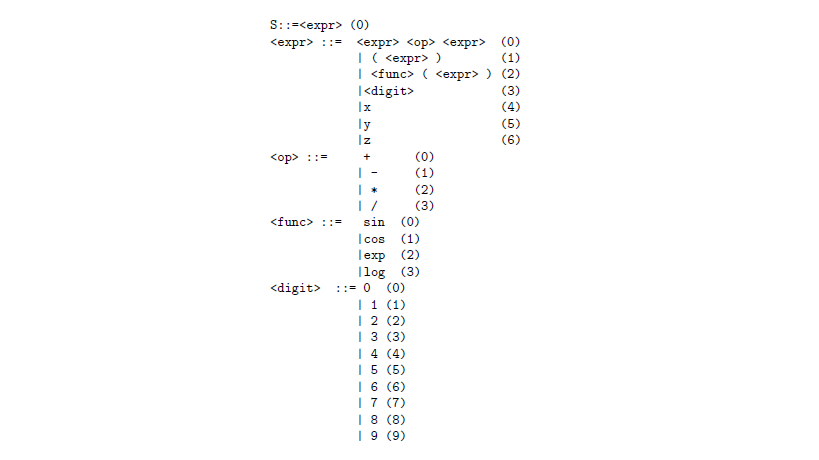
\includegraphics[scale = 0.85]{Pictures/productionRule.png}
%	\caption{\textit{Production rule}}
%	\label{fig:crossover}
%\end{figure}

Simbol S dalam \textit{grammar} menyatakan \textit{start symbol}. Kemudian setiap elemen (gen) kromosom dengan panjang \textit{N} dan berisi bilangan \textit{integer} dari 0 sampai \textit{S} akan diproses di dalam aturan produksi. 

Contoh, ada kromosom \textit{x} = [16, 3, 7, 4, 10, 28, 24, 1, 2, 4]. Pada tabel 1, ditunjukkan bagaimana sebuah fungsi yang valid diproduksi dari \textit{x}. Hasil fungsi menggunakan aturan produksi di gambar 9 menghasilkan \begin{math} f(x) =\log (x^{2}) \end{math}

\begin{table}[H]
\centering
\captionsetup{justification=centering}
\caption{Pembentukan \textit{string}}
\begin{tabular} { | c | c | c | }

\hline
\textit{String} & Kromosom & Operasi \\
\hline 
<expr> & 16, 3, 7, 4, 10, 28, 24, 1, 2, 4 & 16 mod 7 = 2 \\
\hline
<func>(<expr>) & 3, 7, 4, 10, 28, 24, 1, 2, 4 & 3 mod 4 = 3 \\
\hline
log(<expr>) & 7, 4, 10, 28, 24, 1, 2, 4  & 7 mod 7 = 0 \\
\hline
log(<expr><op><expr>) & 4, 10, 28, 24, 1, 2, 4 & 4 mod 7 = 4 \\
\hline
log(x<op><expr>) & 10, 28, 24, 1, 2, 4 & 10 mod 4 = 2 \\
\hline
log(x*<expr>) & 28, 24, 1, 2, 4 & 28 mod 7 = 0 \\
\hline
log(x*<expr><op><expr>) & 24, 1, 2, 4 & 24 mod 7 = 3 \\
\hline
log(x*<digit><op><expr>) & 1, 2, 4 & 1 mod 10=1 \\
\hline
log(x*1<op><expr>) & 2, 4 & 2 mod 4 = 2 \\
\hline
log(x*1*<expr>) & 4 & 4 mod 7 = 4 \\
\hline
log(x*1*x) & & \\
\hline
\end{tabular}
\label{tab:aa}
\end{table}

\subsection{Aplikasi Algoritma Genetik (menggunakan \textit{grammatical evolution}) untuk Mencari Solusi Persamaan Diferensial} %atau lebih baik jadi grammatical evolution
\label{sec:appsAGsolusiPD}

Dalam algoritma genetika untuk mencari solusi persamaaan diferensial biasa dan persamaan diferensial parsial, terjadi proses-proses berikut ini:

\begin{enumerate}[1.]

	\item \textit{Initialization}
	\\
	Pada proses ini, nilai-nilai gen (allele) didefinisikan (dalam kasus ini \textit{allele} bertipe bilangan bulat (\textit{integer})).Nilai untuk \textit{mutation rate} dan \textit{replication rate} ditentukan. \textit{Replication rate} menyatakan pecahan jumlah kromosom yang tidak akan berubah sampai generasi selanjutnya (replikasi). Artinya, peluang untuk kawin silang (\textit{cross}-\textit{over})  ditentukan 1 - \textit{replication rate}. \textit{Mutation rate} mengendalikan rata-rata jumlah perubahan di dalam kromosom. 

	\item \textit{Fitness evaluation}
	\\
	Pada proses ini, nilai \textit{fitness} kromosom-kromosom di populasi akan dievaluasi berdasarkan nilai \textit{fitness}-nya. \textit{Fitness evaluation} untuk persamaan diferensial biasa dan persamaan diferensial parsial adalah sebagai berikut:

	\begin{enumerate}[1.]

		\item Persamaan diferensial biasa
		\\
		Bentuk persamaan diferensial biasa dapat ditunjukkan sebagai berikut ini:
			\begin{equation} f(x, y, y ^{(1)}, ..., y^{(n-1)}, y^{(n)}) = 0, x \in [a, b] \end{equation}
		di mana \begin{math} y^{(n)} \end{math} menyatakan tingkatan (orde) turunan ke-\textit{n} dari \textit{y}. Berikut adalah batasan atau kondisi awal dari:
			\begin{equation} g_i {(x, y, y ^{(1)}, ..., y^{(n-1)})}_{| x = t_i} = 0, i = 1, ..., n \end{equation}
		di mana \begin{math}t_i\end{math} adalah salah satu dari dua titik akhir \textit{a} atau \textit{b}. Langkah-langkah untuk \textit{fitness evaluation} dari populasi adalah sebagai berikut:

		\begin{enumerate}[1.]

			\item Pilih titik ketetanggan (\textit{equidistant point}) \textit{N} \begin{math} (x_0, x_1, ..., x_{(N-1)}) \end{math} di dalam jangkauan (\textit{range}) yang relevan.
			\item Untuk setiap kromosom \textit{i}:

			\begin{itemize}

				\item Susun \textit{corresponding model} (fungsi penalti untuk \textit{equidistant point}) \textit{\begin{math} M_i(x)\end{math}}, yang diekspresikan di dalam \textit{evolutionary grammar} tadi.
				\item Hitung jumlah \textit{corresponding model}:
					\begin{equation} E(M_i) = \sum_{j=0}^{N-1} (f(x_j, M(x_j),..., M_i^{(n)}(x_j))^{2} \end{equation}
				\item Hitung fungsi penalti terkait \begin{math} P(M_i) \end{math} dari persamaan (7)
				\item Hitung nilai \textit{fitness} gabungan dari \textit{corresponding model} dan fungsi penalti terkait dan : 
					\begin{equation} v_i = E(M_i) + P(M_i) \end{equation}
				Fungsi penalti \textit{P} tergantung pada kondisi batasan dan memiliki bentuk persamaan:
					\begin{equation} P(M_i) = \lambda \sum_{k=1}^{n} g^{2}_k(x, M_i, M_i^{(1)},...,M_i^{n-1}|x=t_k) \end{equation}
					di mana \begin{math}\lambda \end{math} adalah sebuah bilangan positif.
			\end{itemize}

		\end{enumerate}

		\item Persamaan diferensial parsial
		\\
		Persamaan diferensial parsial yang dibahas di adalah persamaan diferensial parsial eliptis dengan dua variabel (dua dimensi) dengan kondisi batasan Dirichlet. Persamaan diferensial parsial ini diekspresikan dalam bentuk:
		\begin{equation} f(x, y, \Psi(x, y), \frac{\partial}{\partial x}, \Psi(x, y) \frac{\partial}{\partial y}, \Psi(x, y) \frac{\partial^{2}}{\partial x^{2}}, \Psi(x, y) \frac{\partial^{2}}{\partial y^{2}}) = 0 \end{equation}
		dengan x \begin{math} \in \end{math} \begin{math}  [x_0, x_1] \end{math} x \begin{math}  [y_0, y_1] \end{math}. Kondisi batasan  Dirichlet  yang saling terkait diekspresikan sebagai berikut: \begin{math} \Psi(x_0, y) = f_0(y), \Psi(x_1, y) = f_1(y) = g_0(x), 			\Psi(x, y_1) = g_1(x). \end{math}

		Langkah-langkah untuk \textit{fitness evaluation} dari populasi adalah sebagai berikut:

		\begin{enumerate}[1.]

			\item Pilih \textit{equidistant point} \begin{math} N^{2} \end{math} di dalam \begin{math} [x_0, x_1] \end{math} x \begin{math} [y_0, y_1] \end{math}, \begin{math} N_x \end{math} \textit{equidistant point} pada batas \begin{math} x = x_0 
			\end{math} dan \begin{math} x = x_1 \end{math}, \begin{math} N_y \end{math} \textit{equidistant point} pada batas \begin{math} y = y_0 \end{math} dan \begin{math} y = y_1 \end{math}.
			\item Untuk setiap kromosom \textit{i}:

				\begin{itemize}

					\item Bangun solusi percobaan (\textit{trial solution}) \begin{math} M_i(x, y) \end{math}  yang diekspresikan di dalam \textit{evolutionary grammar} dalam gambar 9.
					\item Hitung jumlah solusi percobaan:

					\begin{equation} E(M_i) = \sum_{j=1}^{N^{2}}f(x_j, y_j, M_i(x_j, y_j), \frac{\partial}{\partial x}Mi(x_j, y_j), \frac{\partial}{\partial y}M_i(x_j, y_j), \frac{\partial^{2}}{\partial x^{2}}M_i(x_j, y_j), \frac{\partial^{2}}{\partial y^{2}}
					M_i(x_j, y_j)^{2} 	\end{equation}

					\item Hitung jumlah-jumlah fungsi penalti terkait:
					\\
					\begin{displaymath} P_1(M_i) = \sum_{j=1}^{N_x}(M_i(x_0,y_j)-f_0(y_j))^{2} \end{displaymath}
					\\
					\begin{displaymath} P_2(M_i) = \sum_{j=1}^{N_x}(M_i(x_1,y_j)-f_1(y_j))^{2} \end{displaymath}
					\\
					\begin{displaymath} P_3(M_i) = \sum_{j=1}^{N_y}(M_i(x_j,y_0)-g_0(x_j))^{2} \end{displaymath}
					\\
					\begin{displaymath} P_4(M_i) = \sum_{j=1}^{N_y}(M_i(x_j,y_1)-g_1(x_j))^{2} \end{displaymath}

					\item Hitung \textit{fitness} kromosom:

					\begin{equation} v_i = E(M_i) +\lambda(P_1(M_i)+P_2(M_i)+P_3(M_i)+P_4(M_i)) \end{equation}

				\end{itemize}

		\end{enumerate}

\end{enumerate}

Contoh \textit{fitness evaluation} untuk persamaan diferensial biasa:
\\
Terdapat sebuah persamaan diferensial biasa sebagai berikut:

	\begin{displaymath} y''+100y = 0, x \in [0, 1] \end{displaymath}

dengan kondisi batasan \begin{math}y(0) = 0 \end{math} dan \begin{math}y'(0) = 10 \end{math}. \textit{Range} yang diambil [0, 1] \textit{N} = 10 \textit{equidistant point} \begin{math} x_0, ..., x_9 \end{math}. Terdapat kromosom-kromosom dengan panjang 10 dalam populasi dan salah satu kromosom di dalam populasi adalah \textit{g} = [7, 2, 10, 4, 4, 2, 11, 8, 18, 30, 5]. Mengacu pada aturan produksi yang ada pada gambar 3 tentang \textit{evolutionary grammar}, fungsi yang berkorespondensi dengan kromosom \textit{g} adalah \begin{math} M_g(x) = exp(x) + \sin (x) \end{math}. Turunan pertama adalah \begin{math} M_g^{(1)(x)} = exp(x) + \cos (x) \end{math} dan turunan kedua adalah \begin{math} M_g^{(2)(x)} = exp(x) - \sin (x) \end{math}. 
\\
Dengan persamaan 6 didapat:

	\begin{displaymath} E(M_g) = \sum_{i=0}^{9}(M_g^{(2)}(x_i)+100M_g(x_i))^{2} \end{displaymath}
\\
	\begin{displaymath} E(M_g) = \sum_{i=0}^{9}(101exp(x_i)+99sin(x_i))^{2}\end{displaymath}
\\
	\begin{displaymath} E(M_g) = 484933.2 \end{displaymath}

\textit{Penalty function} \begin{math}P(M_g) \end{math} dihitung sesuai persamaan 8 adalah:
	
	\begin{displaymath} P(M_g) = \lambda(M_g(0)-y(0))^{2}+(M_g^{(1)}(0)-y''(0))^{2} \end{displaymath}
	\begin{displaymath} P(M_g) = \lambda(exp(0)+sin(0)+0)^{2}+(exp(0)-sin(0)-10)^{2} \end{displaymath}
	\begin{displaymath} P(M_g) = \lambda(1+0-0)^{2}+(1-0-10)^{2} \end{displaymath}
	\begin{displaymath} P(M_g) = 82\lambda \end{displaymath}

Jadi \textit{fitness value} \begin{math} u_g \end{math} dari kromosom yang diberikan adalah:

\begin{displaymath} u_g = E(M_g)+P(M_g)\end{displaymath}
\begin{displaymath} u_g =  484933.2 + 82\lambda \end{displaymath}

Kemudian \textit{fitness value} setiap kromosom akan diurutkan menaik dari yang terkecil hingga terbesar. Lalu, \textit{genetic operator} akan dipakai, lalu populasi baru akan tercipta. dan proses ini diulang sampai kriteria proses \textit{termination} terpenuhi.

\item \textit{Genetic operations}
\\
Operator genetik yang diaplikasikan pada populasi genetik adalah \textit{initialization}, kawin silang (\textit{cross}-\textit{over}), dan mutasi. \textit{Initialization} hanya diaplikasikan hanya sekali pada generasi pertama saja. Untuk setiap elemen pada setiap kromosom, bilangan \textit{integer} acak pada \textit{range} tertentu dipilih.
\\
Kawin silang diaplikasikan pada setiap generasi supaya kromosom baru dapat tercipta dari kromosom yang lama, yang akan mengganti individu-individu dalam populasi. Setiap pasangan dari kromosom baru, dua induk dipilih. Kedua induk ini "dipotong" pada titik terpilih secara acak
dan masing-masing sub-kromosom pada sisi sebelah kanan ditukar. Contoh:

%masukkin gambar cross-over one point
%
%\begin{figure}[H]
%\centering
%\captionsetup{justification = centering}
%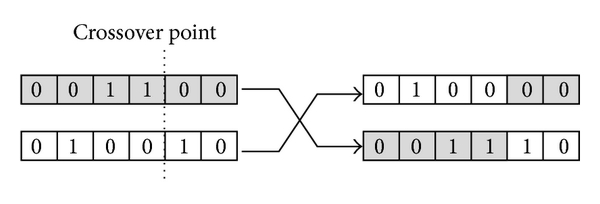
\includegraphics[scale = 1.5]{Pictures/crossover1Point.png}
%\caption{\textit{cross}-{over} 1 \textit{point}}
%\label{fig:crossover}
%\end{figure}

Induk dipilih melalui seleksi turnamen sebagai berikut ini:
\begin{itemize}
	\item Pertama, buat grup individu yang terpilih secara acak dengan jumlah \textit{K} \begin{math} \geq \end{math} 2 dari populasi terkini.
	\item Individu dengan \textit{fitness} terbaik dalam grup dipilih
\end{itemize}

Pada setiap generasi, langkah-langkah berikut ini dilakukan:
\begin{enumerate}[1.]
	\item Kromosom-kromosom diurutkan berdasarkan \textit{fitness value}-nya, dengan cara kromosom terbaik ditempatkan di awal populasi, sedangkan kromosom terburuk di akhir populasi.
	\item \begin{math} c = (1 - s) * g \end{math} kromosom baru diproduksi oleh operasi \textit{cross}-\textit{over}, di mana \textit{s} adalah \textit{replication rate} dari model populasi dan \textit{g} jumlah total individual di dalam populasi. Individual-individual baru akan menggantikan individual-individual terburuk di populasi pada saat operasi \textit{cross}-\textit{over} berakhir.
	\item Operasi mutasi diaplikasikan kepada setiap kromosom, di luar yang sudah dipilih untuk replikasi pada generasi selanjutnya.
\end{enumerate}

\item \textit{Termination control}
\\
\textit{Termination control} adalah proses algoritma genetik selesai dijalankan. Proses ini terjadi apabila salah satu dari kedua hal ini terjadi:
	\begin{enumerate}[1.]
		\item Iterasi pada gen-gen kromosom sudah mencapai angka maksimum yang ditentukan
		\item Sudah mencapai ambang batas (\textit{threshold}) yang ditentukan (solusi sudah ditemukan)
		\item Tidak ada lagi perkembangan yang terjadi
	\end{enumerate}

\end{enumerate}
